\PassOptionsToPackage{T5,T1}{fontenc}
\documentclass{template}

% -----------------------------------------------------------------------------
% PROJECT METADATA -- edit these values first.
% -----------------------------------------------------------------------------
\newcommand{\ProjectName}{Super Mario Flashback}
\newcommand{\GroupID}{5}
\newcommand{\CourseName}{CS202 -- Programming Systems}
\newcommand{\ClassName}{25A02}
\newcommand{\LecturerName}{PhD. Dinh Ba Tien}
\newcommand{\TeachingAssistants}{Ho Tuan Thanh; Truong Phuoc Loc}
\newcommand{\SemesterName}{Semester 3, 2026}
\newcommand{\VN}[1]{{\fontencoding{T5}\fontfamily{cmr}\selectfont #1}}

% Keep this switch true while writing. Change it to \reportdraftfalse before
% submitting to hide all yellow TODO boxes.
\newif\ifreportdraft
\reportdraftfalse

\definecolor{mariored}{HTML}{D32F2F}
\definecolor{marioblue}{HTML}{1565C0}
\definecolor{mariogold}{HTML}{F9A825}
\definecolor{mariogreen}{HTML}{2E7D32}
\definecolor{gamelight}{HTML}{FFF8E1}
\definecolor{gamegray}{HTML}{607D8B}
\definecolor{codebackground}{HTML}{F7F9FC}
\definecolor{codeborder}{HTML}{B8C2CC}

\hypersetup{
    colorlinks=true,
    linkcolor=marioblue,
    urlcolor=marioblue,
    citecolor=marioblue,
    pdftitle={\ProjectName{} Final Project Report},
    pdfauthor={Group \GroupID}
}

\usepackage{tabularx}
\usetikzlibrary{arrows.meta,positioning,shapes.geometric,fit}

\lstdefinestyle{gamecode}{
    language=C++,
    backgroundcolor=\color{codebackground},
    basicstyle=\ttfamily\footnotesize,
    breaklines=true,
    captionpos=b,
    columns=fullflexible,
    commentstyle=\color{mariogreen},
    frame=single,
    identifierstyle=\color{black},
    keepspaces=true,
    keywordstyle=\color{marioblue}\bfseries,
    numbers=left,
    numbersep=8pt,
    numberstyle=\tiny\color{gamegray},
    rulecolor=\color{codeborder},
    showspaces=false,
    showstringspaces=false,
    stringstyle=\color{codepurple},
    tabsize=4
}

\newcommand{\ReportTODO}[1]{%
    \ifreportdraft
        \par\smallskip
        \noindent\fcolorbox{mariogold}{gamelight}{%
            \parbox{\dimexpr\linewidth-2\fboxsep-2\fboxrule\relax}{%
                \textbf{TODO:} #1}}
        \par\smallskip
    \fi
}

\newcommand{\ReportFigure}[3]{%
    \begin{figure}[H]
        \centering
        \IfFileExists{#1}{%
            \includegraphics[width=0.9\textwidth]{#1}%
        }{%
            \fcolorbox{gamegray}{white}{%
                \parbox[c][5.2cm][c]{0.86\textwidth}{%
                    \centering
                    \textcolor{gamegray}{\Large Figure placeholder}\par
                    \vspace{0.35cm}
                    Add \texttt{\detokenize{#1}} to the project.}}
        }
        \caption{#2}
        \label{#3}
    \end{figure}
}

\tikzset{
    architecture/.style={
        draw=gamegray,
        fill=white,
        rounded corners=2pt,
        line width=0.8pt,
        minimum width=3.5cm,
        minimum height=1.05cm,
        align=center,
        font=\sffamily\small
    },
    architecturearrow/.style={
        -{Stealth[length=2.6mm]},
        draw=gamegray,
        line width=0.8pt
    },
    patternnode/.style={
        draw=gamegray,
        fill=white,
        rounded corners=2pt,
        line width=0.75pt,
        minimum width=2.7cm,
        minimum height=0.9cm,
        align=center,
        font=\sffamily\scriptsize
    },
    patterninterface/.style={
        patternnode,
        fill=marioblue!7
    },
    patternhighlight/.style={
        patternnode,
        fill=mariogold!13
    },
    patternarrow/.style={
        -{Stealth[length=2.7mm]},
        draw=marioblue,
        line width=0.85pt
    },
    patternuses/.style={
        -{Stealth[length=2.5mm]},
        draw=gamegray,
        dashed,
        line width=0.75pt
    },
    patterninherit/.style={
        -{Triangle[open,length=3mm,width=3mm]},
        draw=gamegray,
        line width=0.8pt
    }
}

\setcounter{tocdepth}{2}
\setcounter{secnumdepth}{3}

\begin{document}

% =============================================================================
% COVER PAGE
% =============================================================================
\pagenumbering{gobble}
\begin{titlepage}
    \centering
    \vspace*{-0.6cm}

    \includegraphics[width=10.5cm]{hcmus-logo.png}\par
    \vspace{0.2cm}

    {\fontsize{20}{23}\selectfont\bfseries FINAL PROJECT REPORT\par}
    \vspace{0.75cm}
    {\fontsize{32}{36}\selectfont\bfseries\color{mariored}
        \MakeUppercase{\ProjectName}\par}
    \vspace{1cm}

    \begin{tabular}{@{}rl@{}}
        \textbf{Group ID:} & \GroupID \\
        \textbf{Course:} & \CourseName \\
        \textbf{Class:} & \ClassName \\
        \textbf{Lecturer:} & \LecturerName \\
        \textbf{Teaching Assistants:} & \TeachingAssistants \\
        \textbf{Semester:} & \SemesterName \\
        \textbf{Last modified:} & \today
    \end{tabular}

    \vspace{1cm}
    {\Large\bfseries Group Members\par}
    \vspace{0.15cm}

    {\fontencoding{T5}\fontfamily{cmr}\selectfont
    \begin{tabular}{@{}cl@{}}
        \toprule
        \textbf{Student ID} & \textbf{Name} \\
        \midrule
        25125015 & Nguyễn Phạm Đức Huy \\
        25125018 & Nguyễn Minh Khang \\
        25125034 & Trần Quyết Thắng \\
        25125052 & Võ Thành Đạt \\
        \bottomrule
    \end{tabular}}
\end{titlepage}

% =============================================================================
% FRONT MATTER
% =============================================================================
\pagenumbering{roman}

\section*{Document Status}
\addcontentsline{toc}{section}{Document Status}

\begin{tabularx}{\textwidth}{@{}lX@{}}
    \toprule
    \textbf{Item} & \textbf{Information} \\
    \midrule
    Source repository & Project source archive supplied with the report;
    repository URL and submission commit/tag were not present in the available
    materials. \\
    Demo video & \url{https://youtu.be/EXjN6fgQRZw?si=Lmf81SBxOXa-5IpL} \\
    Executable/release & \url{https://youtu.be/EXjN6fgQRZw?si=Lmf81SBxOXa-5IpL} build
    instructions are provided in Appendix~A. \\
    Target platform & 64-bit Windows 10 or Windows 11. \\
    Graphics library & SFML 2.x; the exact patch version is not recorded in the
    available project files. \\
    Report version & v1.0 submission candidate, September 2, 2026. \\
    \bottomrule
\end{tabularx}

\section*{Abstract}
\addcontentsline{toc}{section}{Abstract}

\textit{Super Mario Flashback} is a non-commercial two-dimensional
side-scrolling platform game developed as the final project for CS202. The game
was implemented in C++17 with SFML 2.x and CMake, without using a complete game
engine. It provides a continuous single-player experience from menu and
character selection through movement, jumping, collision, enemies, items,
audio, saving, level completion, and game-over states. Mario and Luigi are
selectable characters with distinct movement parameters. Three hand-authored
campaign levels introduce grassland, cave, and castle environments with
increasing traversal and combat difficulty; generated and pipe-based levels
provide supplementary content.

The software applies object-oriented principles through reusable state, player,
enemy, item, movement, renderer, and service abstractions. Factory, Singleton,
Observer, State, and Strategy are the five primary design patterns, while
Command and Template Method support input handling and shared item behavior.
Text-based level data, centralized resource management, event-based gameplay
responses, and versioned persistence keep major responsibilities separated.
Independent checks confirmed the structure of all five supplied level files
and the core save/load validation paths. The principal result is an integrated
platform-game architecture that supports multiple themes and entity behaviors
without duplicating the main execution loop. Final GUI regression testing and
quantitative performance measurements remain release-verification tasks.

\section*{Acknowledgements}
\addcontentsline{toc}{section}{Acknowledgements}

The team thanks Dr. Dinh Ba Tien and teaching assistants Ho Tuan Thanh and
Truong Phuoc Loc for their instruction and feedback during the CS202 course.
The team also acknowledges classmates and testers who provided gameplay and
integration feedback. Third-party visual and font resources remain the
property of their respective creators and rights holders, as detailed in
Section~12.

\clearpage
\tableofcontents
\clearpage
\listoffigures
\addcontentsline{toc}{section}{List of Figures}
\listoftables
\addcontentsline{toc}{section}{List of Tables}
\clearpage

\pagenumbering{arabic}

% =============================================================================
% MAIN REPORT
% =============================================================================
\section{Introduction}

\subsection{Background and Motivation}

\textit{Super Mario Flashback} is a two-dimensional side-scrolling platform
game developed by Group~\GroupID{} as the final project for \CourseName. The
project was implemented in C++17 with SFML~2 and CMake, without relying on a
complete game engine. Its purpose is to combine the programming topics studied
in the course into a real-time application in which input processing, physics,
rendering, audio, user-interface transitions, resource ownership, and
persistent data must operate together consistently.

A platform game is particularly suitable for demonstrating object-oriented
design because its world contains many objects that share common interfaces
but require different behavior. Mario and Luigi reuse a player abstraction
while retaining different movement characteristics; enemies and collectible
items are processed polymorphically; movement algorithms are separated from
enemy types; and menus, gameplay, pause, game-over, and level-complete screens
have independent state behavior. The project therefore provides concrete
reasons to apply encapsulation, inheritance, abstraction, polymorphism, and
design patterns instead of presenting them only as isolated examples.

The game also gives the team experience with practical software-engineering
concerns beyond basic gameplay. Levels are loaded from validated text files,
game objects are created through factories, frequently used SFML resources are
cached, and progress can be saved and restored through a versioned local file.
These decisions support maintainability and extension while keeping the
gameplay code separate from data parsing and infrastructure services.

This project is a non-commercial educational work inspired by the conventions
of classic platform games. The team does not claim ownership of Super Mario,
Nintendo characters, or other third-party intellectual property used as study
references or credited assets.

\subsection{Project Objectives}

The project has the following objectives:

\begin{itemize}
    \item deliver a complete single-player platform-game loop with responsive
          movement, jumping, animation, camera tracking, tile collision, pit
          detection, scoring, lives, a countdown timer, and clear win and loss
          conditions;
    \item provide three progressively difficult campaign levels, bonus pipe
          sub-levels, and an optional procedurally generated level mode with
          selectable difficulty;
    \item support Mario and Luigi as selectable characters with distinct
          movement parameters, together with enemies, projectiles, a boss
          encounter, coins, and multiple power-up types;
    \item demonstrate the four principal OOP concepts through reusable player,
          enemy, item, strategy, renderer, state, and user-interface
          abstractions;
    \item apply design patterns---including State, Strategy, Factory,
          Observer, Singleton, Template Method, and Command---to actual
          architectural problems in the game;
    \item keep level parsing, object construction, gameplay rules, resource
          management, audio, and persistence in separate modules so that new
          content can be added with limited changes to existing code; and
    \item provide menu and pause flows, configurable audio and key bindings,
          level unlocking, versioned save/load support, and sufficient
          documentation for building, using, and evaluating the project.
\end{itemize}

\subsection{Scope and Limitations}

\begin{tabularx}{\textwidth}{@{}p{0.23\textwidth}X@{}}
    \toprule
    \textbf{Category} & \textbf{Declared scope} \\
    \midrule
    In scope & A Windows-oriented, single-player 2D platform game; Mario and
    Luigi character selection; three hand-authored campaign levels; a
    difficulty-based random level generator; pipe sub-levels; player movement,
    animation, camera, and tile collision; Goomba, Koopa, flying, Hammer Bro,
    and boss enemies; projectiles and Koopa-shell interactions; coins and six
    item or power-up types; HUD, menu, level-select, options, pause, game-over,
    and completion screens; music and sound effects; configurable controls;
    level unlocking; and local save/load persistence. \\
    Out of scope & Simultaneous multiplayer and networking, mobile/web/console
    ports, a three-dimensional mode, a graphical level editor, user accounts or
    cloud saves, and commercial distribution. \\
    Known limitations & The supplied build configuration and SFML runtime are
    centered on Windows. Assets and maps are loaded through an expected
    relative directory structure. Persistence uses one local plain-text save
    slot, while the random mode regenerates a single map file rather than
    providing seed sharing, editing, or long-term storage of generated levels. \\
    \bottomrule
\end{tabularx}

\subsection{Team Contributions}

\begin{longtable}{@{}p{2.2cm}p{3.4cm}p{7.5cm}p{1.8cm}@{}}
    \caption{Summary of team contributions.}\label{tab:contributions}\\
    \toprule
    \textbf{Student ID} & \textbf{Name} & \textbf{Main responsibilities} &
    \textbf{Share} \\
    \midrule
    \endfirsthead
    \toprule
    \textbf{Student ID} & \textbf{Name} & \textbf{Main responsibilities} &
    \textbf{Share} \\
    \midrule
    \endhead
    25125015 & \VN{Nguyễn Phạm Đức Huy} & Overall architecture; state, event,
    resource, audio, camera, persistence, procedural-map, pipe sub-level, and
    level-progression systems; data validation; project documentation. &
    See form \\
    25125018 & \VN{Nguyễn Minh Khang} & Level design and difficulty tuning;
    castle scenery and exit sequence; Koopa shell--wall collision edge cases. &
    See form \\
    25125034 & \VN{Trần Quyết Thắng} & Enemy and boss systems; Hammer Bro and
    projectile behavior; Koopa shell state mechanics; collision fixes;
    invincibility, pipe, and gameplay-audio integration. & See form \\
    25125052 & \VN{Võ Thành Đạt} & Menu and UI refinement; enemy-system
    refactoring; initial boss integration; shell-carry animation assets and
    related code cleanup. & See form \\
    \bottomrule
\end{longtable}

The table records the main ownership areas found in the project documentation.
Because many features were integrated and debugged collaboratively, the final
quantitative contribution shares are reported separately in the required group
evaluation form rather than estimated in this report.

\clearpage
\section{Requirements and Game Overview}

\subsection{Game Concept}

\textit{Super Mario Flashback} is a single-player side-scrolling platform game
whose main goal is to guide Mario or Luigi through a sequence of increasingly
difficult stages. The project does not depend on an elaborate narrative; its
premise follows the familiar structure of a platform adventure in which the
player crosses hazardous terrain, collects useful items, defeats enemies, and
reaches the level exit. It is intended both for course evaluation and for
players who are familiar with accessible keyboard-based platform games.

At the beginning of a new session, the player selects Mario or Luigi and then
chooses an unlocked campaign level or the random-level mode. During gameplay,
the repeated loop consists of moving and jumping through the map, avoiding
pits and projectiles, interacting with question blocks and pipes, collecting
coins and power-ups, and deciding whether to stomp, evade, or use a Koopa shell
against enemies. The HUD continuously reports the current world, score, lives,
coin count, power state, temporary effects, and remaining time.

A campaign level is completed by reaching its exit pole. Finishing Levels 1
and 2 unlocks and loads the next level, while the exit in Level 3 remains
closed until the boss is defeated. Falling into a pit, taking damage without a
protective power state, or allowing the timer to expire costs a life; reaching
zero lives opens the game-over state. Defeating the final boss and completing
Level 3 produces the victory state. Character-specific movement, data-driven
levels, generated stages, pipe sub-levels, varied enemy behavior, and
persistent progress distinguish the project from a minimal platform-game
prototype.

\subsection{Functional Requirements}

\begin{longtable}{@{}p{1.1cm}p{3.2cm}p{7.3cm}p{2.4cm}@{}}
    \caption{Functional requirements.}\label{tab:functional-requirements}\\
    \toprule
    \textbf{ID} & \textbf{Requirement} & \textbf{Acceptance evidence} &
    \textbf{Status} \\
    \midrule
    \endfirsthead
    \toprule
    \textbf{ID} & \textbf{Requirement} & \textbf{Acceptance evidence} &
    \textbf{Status} \\
    \midrule
    \endhead
    FR-01 & Player input and movement & \texttt{Player} reads configurable
    movement and action bindings, supports arrow-key alternatives, applies
    acceleration damping, gravity, jump buffering, and coyote time, and drives
    character animation states. & Implemented \\
    FR-02 & Collision and world boundaries & \texttt{TileMap::resolveCollision}
    resolves horizontal and vertical tile contact separately. Gameplay also
    detects pits, solid map boundaries, enemies, items, projectiles, question
    blocks, and exit triggers. & Implemented \\
    FR-03 & Enemy behavior & \texttt{EnemyFactory} creates Goomba, Koopa,
    FlyingEnemy, HammerBro, and BossEnemy objects with patrol, chase, flying, or
    boss behavior. Koopa shells and enemy projectiles provide additional
    interactions. & Implemented \\
    FR-04 & Items and power-ups & \texttt{ItemFactory} supports Coin,
    Mushroom, FireFlower, OneUpMushroom, Star, and SpeedBoost. Their events
    update score, lives, power state, invincibility, movement speed, audio, and
    HUD feedback. & Implemented \\
    FR-05 & Campaign levels and progression & The validated files
    \texttt{levels/level1.txt} through \texttt{level3.txt} provide Easy,
    Medium, and Hard stages. Exit handling unlocks the next level and gates the
    final exit while the boss is active. & Implemented \\
    FR-06 & Music and sound effects & \texttt{AudioManager} provides
    background music and effects for jumping, coins, power-ups, extra lives,
    temporary abilities, enemy defeat, fireballs, pipes, and game over. &
    Implemented \\
    FR-07 & Menus and game states & Concrete \texttt{GameState} classes cover
    the main menu, character and level selection, random generation, options,
    gameplay, pause, game over, level completion, and about screens. &
    Implemented \\
    FR-08 & HUD, score, lives, and timer & \texttt{GameHud} displays world,
    score, lives, coins, power state, effect timers, and remaining time. Events
    update values and show short status messages during play. & Implemented \\
    FR-09 & Save and load & The version-1 save format stores the current and
    highest unlocked levels, score, lives, character, position, power state,
    time, and coins. Invalid or incompatible files are rejected safely. &
    Implemented \\
    FR-10 & Character selection & \texttt{CharacterSelectState} offers Mario
    and Luigi. Both use the shared \texttt{Player} abstraction, while their
    movement speed, jump power, dimensions, and animations differ. &
    Implemented \\
    FR-11 & Generated and pipe levels & \texttt{MapGenerator} creates an Easy,
    Medium, or Hard random stage in \texttt{level4.txt}. Entering a supported
    pipe generates or restores a compact cached sub-level through
    \texttt{level5.txt}. & Implemented \\
    FR-12 & Configurable settings & \texttt{OptionsState} changes difficulty,
    BGM and SFX volume, and keyboard bindings. \texttt{SettingsManager} saves
    these values in \texttt{settings.txt} and can restore defaults. &
    Implemented \\
    \bottomrule
\end{longtable}

\subsection{Non-Functional Requirements}

\begin{itemize}
    \item \textbf{Performance:} The application targets 60 updates and rendered
          frames per second using a fixed $1/60$-second simulation step and a
          1920-by-1080 logical view. Batched tile geometry and cached textures,
          fonts, and sound buffers reduce repeated work during gameplay. These
          values are implementation targets rather than hardware benchmark
          results.
    \item \textbf{Usability:} The game supports mouse-driven menus, keyboard
          shortcuts, remappable gameplay keys, separate BGM/SFX volume controls,
          a readable HUD, status notifications, and consistent pause, restart,
          back, and exit actions.
    \item \textbf{Reliability:} Level files are validated before use, including
          metadata, dimensions, symbols, and required spawn data. Save files
          are range-checked and version-checked; writes use a temporary file
          and backup procedure so a failed write does not silently replace a
          valid save.
    \item \textbf{Maintainability:} Interfaces and module boundaries separate
          states, entities, factories, levels, events, resources, audio,
          persistence, camera, and UI code. Smart-pointer ownership and
          data-driven object spawning limit manual lifetime management and
          reduce changes required when adding content.
    \item \textbf{Portability:} The CMake project contains configurations for
          Microsoft Visual C++ and MinGW-w64 on Windows 10/11. It copies the
          required SFML runtime files, assets, and levels beside the executable.
          Other operating systems are not part of the declared tested scope.
\end{itemize}

\subsection{Controls}

\begin{table}[H]
    \centering
    \caption{Player controls.}
    \label{tab:controls}
    \begin{tabularx}{\textwidth}{@{}p{3.4cm}p{4.4cm}X@{}}
        \toprule
        \textbf{Action} & \textbf{Keyboard input} &
        \textbf{Notes} \\
        \midrule
        Move left/right & A/D by default; Left/Right arrows & A/D can be
        rebound. Mario and Luigi have different horizontal speeds. \\
        Jump & W or Space by default; Up arrow & The Move Up and Action
        bindings can be changed. Jump buffering and coyote time improve input
        tolerance. \\
        Fire or handle Koopa shell & Z & Fire-form characters shoot on press.
        Holding Z while touching an idle shell picks it up; releasing Z throws
        it. \\
        Enter or leave a pipe & Down arrow & Works while standing on a
        compatible pipe and uses a short transition and cooldown. \\
        Pause/resume & Escape by default or the HUD menu button & The pause key
        can be rebound; the pause menu also opens Options or returns to the main
        menu. \\
        Quick save/load & F5/F9 & Saves the current session or reloads the
        validated local save file. \\
        Menu navigation & Mouse; arrows or A/D; Enter/Space; Escape & Exact
        alternatives depend on the active menu. Number keys 1--3 select unlocked
        campaign levels and 4 opens random generation. \\
        Restart/return after result & R; Enter & R restarts after game over or
        victory; Enter returns to the main menu after victory. \\
        \bottomrule
    \end{tabularx}
\end{table}

\subsection{Level Progression}

\begin{table}[H]
    \centering
    \caption{Level progression and increasing difficulty.}
    \label{tab:levels}
    \begin{tabularx}{\textwidth}{@{}lXXX@{}}
        \toprule
        \textbf{Level} & \textbf{Theme and goal} & \textbf{Mechanics/enemies} &
        \textbf{Difficulty increase} \\
        \midrule
        Level 1 & Easy field stage focused on reaching the first exit. & Broad
        ground sections, coins, question blocks, Goombas, Koopas, and pipes. &
        Establishes movement, jumping, collection, and basic enemy interaction
        with comparatively forgiving terrain. \\
        Level 2 & Medium athletic or broken-bridge stage with more demanding
        traversal. & More separated platforms and pits, a denser enemy mix,
        flying enemies, and additional pipe positions. & Requires more precise
        jumps and combines airborne and ground threats. \\
        Level 3 & Hard castle stage culminating in the final exit and boss
        encounter. & Castle-themed terrain, tighter obstacle placement, more
        Koopas and flying enemies, projectiles, and a boss-gated exit. & Combines
        the previous mechanics and requires the boss to be defeated before the
        campaign can be completed. \\
        \bottomrule
    \end{tabularx}
\end{table}

Outside the ordered campaign, the Random option asks for an Easy, Medium, or
Hard difficulty and writes a newly generated stage to \texttt{level4.txt}.
Pipes may lead to a shorter generated sub-level stored in \texttt{level5.txt};
the sub-level is cached for the active pipe so that returning to it during the
same session restores the same layout and then returns the player to the main
stage.

\clearpage
\section{Technology Stack and Development Environment}

The game is implemented directly on top of C++ and SFML rather than a complete
game engine. Table~\ref{tab:technology-stack} summarizes the technologies that
are required to build the program and the project-specific role of each one.
The language, library, and build-system terminology follows the documentation
listed in References~3--6.

\begin{table}[H]
    \centering
    \caption{Development technology stack.}
    \label{tab:technology-stack}
    \begin{tabularx}{\textwidth}{@{}p{3.5cm}XX@{}}
        \toprule
        \textbf{Technology} & \textbf{Version/configuration} &
        \textbf{Role in the project} \\
        \midrule
        C++ language & C++17, enforced by \texttt{CMAKE\_CXX\_STANDARD} & Core
        OOP implementation, standard containers, smart pointers,
        \texttt{std::optional}, and filesystem operations. \\
        Graphics and multimedia & SFML 2.x, using Graphics, Window, System, and
        Audio facilities & Window creation, event and keyboard input, sprites,
        text, shapes, views, timing, music, and sound effects. \\
        Build system & CMake 3.15 or newer; MSVC and MinGW-w64 configurations &
        Source discovery, compiler configuration, linking, runtime-file copying,
        and optional CTest targets. \\
        Physics and collision & Custom fixed-step character and tile physics &
        Gravity, velocity, axis-separated tile resolution, world bounds, pits,
        enemy/item contact, projectiles, and shell interactions. \\
        Level and persistence data & Validated plain-text map files and
        version-1 key--value save files & Editable level metadata and tile grids;
        storage of progress, player state, position, score, lives, time, and
        settings. \\
        Development and documentation & Windows 10/11, Visual Studio 2022 or
        MinGW-w64, Git, Mermaid, and LaTeX & Compilation, version control,
        architecture diagrams, and preparation of the final technical report. \\
        \bottomrule
    \end{tabularx}
\end{table}

C++17 provides the language features needed for the project's ownership and
abstraction model without introducing a dependency on newer compiler modes.
In particular, \texttt{std::unique\_ptr} expresses exclusive ownership of
states and game objects, \texttt{std::optional} represents a validated or
missing save, and virtual interfaces support polymorphic entities, strategies,
renderers, commands, and game states. SFML supplies the multimedia primitives
needed by a 2D game while leaving the update loop, collision rules, object
model, and architectural patterns visible for assessment.

CMake makes the source layout usable with both Visual Studio and MinGW-w64 and
copies the relative \texttt{assets/} and \texttt{levels/} directories beside
the executable. At runtime, \texttt{GameManager} uses a fixed $1/60$-second
update step, a 60 FPS limit, and a 1920-by-1080 logical view that is adjusted to
the current window aspect ratio. The project uses custom physics rather than an
external physics engine because the required platform-game collision behavior
is limited enough to implement directly and forms part of the programming
exercise.

Plain-text formats were selected for levels, saves, and settings because they
are easy to inspect, edit, debug, and validate. The level loader converts map
symbols into neutral spawn requests, while factories decide which concrete
objects to construct. Save data is written with an explicit version and a
temporary-file procedure, providing a simple migration and recovery boundary.
Because the available materials identify only SFML~2.x, the final archive
should retain the bundled binaries for reproducibility.

\clearpage
\section{System Architecture}

\subsection{Architectural Overview}

The application uses a state-centered architecture built around
\texttt{GameManager}. This manager owns the SFML window, the stable screen
view, the application settings, and a vector of
\texttt{std::unique\_ptr<GameState>} values that is operated as a stack. It
polls input, advances the fixed-step update loop, renders the required states,
and applies push, pop, or replacement requests. Input and updates are sent only
to the top state, while overlay states such as Pause can be rendered above the
state beneath them.

Concrete states isolate the behavior of menus, selection screens, options,
gameplay, and result screens. \texttt{PlayState} is the central coordinator for
an active game session: it owns the player, enemies, items, projectiles, tile
map, camera, HUD, transient effects, and current \texttt{SaveData}. It invokes
the relevant subsystem in a controlled order but does not implement every
responsibility itself. Collision geometry remains in \texttt{TileMap}, object
construction remains in factories, assets remain in \texttt{ResourceManager},
and sound playback remains in \texttt{AudioManager}.

\begin{figure}[H]
    \centering
    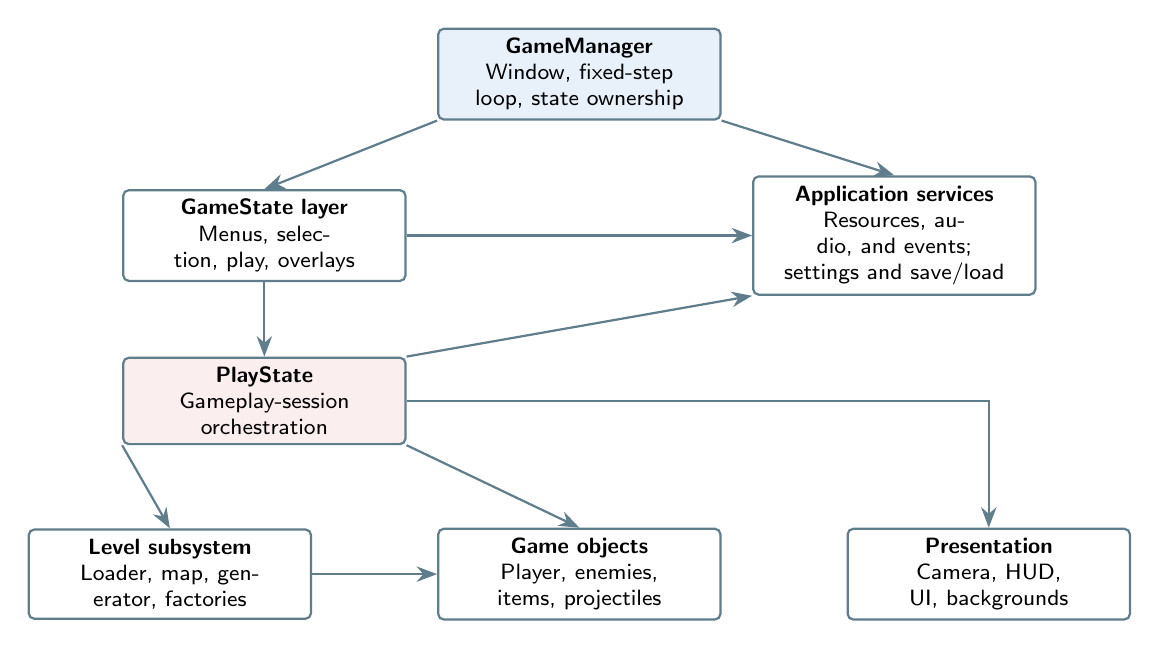
\begin{tikzpicture}[
        archsmall/.style={architecture,minimum width=3.35cm,
                         text width=3.35cm,minimum height=0.95cm,
                         font=\sffamily\footnotesize}
    ]
        \node[archsmall,fill=marioblue!10] (manager) at (0,0)
            {\textbf{GameManager}\\Window, fixed-step loop, state ownership};
        \node[archsmall] (states) at (-4.0,-2.05)
            {\textbf{GameState layer}\\Menus, selection, play, overlays};
        \node[archsmall] (services) at (4.0,-2.05)
            {\textbf{Application services}\\Resources, audio, and events;\\
             settings and save/load};
        \node[archsmall,fill=mariored!8] (play) at (-4.0,-4.15)
            {\textbf{PlayState}\\Gameplay-session orchestration};
        \node[archsmall] (levels) at (-5.2,-6.35)
            {\textbf{Level subsystem}\\Loader, map, generator, factories};
        \node[archsmall] (objects) at (0,-6.35)
            {\textbf{Game objects}\\Player, enemies, items, projectiles};
        \node[archsmall] (presentation) at (5.2,-6.35)
            {\textbf{Presentation}\\Camera, HUD, UI, backgrounds};

        \draw[architecturearrow] (manager.south west) -- (states.north);
        \draw[architecturearrow] (manager.south east) -- (services.north);
        \draw[architecturearrow] (states.east) -- (services.west);
        \draw[architecturearrow] (states.south) -- (play.north);
        \draw[architecturearrow] (play.south west) -- (levels.north);
        \draw[architecturearrow] (play.south east) -- (objects.north);
        \draw[architecturearrow] (play.east) -| (presentation.north);
        \draw[architecturearrow] (play.north east) -- (services.south west);
        \draw[architecturearrow] (levels.east) -- (objects.west);
    \end{tikzpicture}
    \caption{High-level architecture and principal dependency directions.}
    \label{fig:architecture}
\end{figure}

Level construction follows a two-stage data flow. \texttt{TileMap} asks
\texttt{LevelLoader} to validate a text file and return \texttt{LevelData},
including neutral \texttt{LevelSpawnRequest} records. \texttt{PlayState} then
passes these requests to \texttt{LevelObjectFactory}, which delegates to the
enemy or item factory and returns polymorphic objects. Consequently, the parser
does not depend on concrete classes such as \texttt{Goomba} or
\texttt{FireFlower}, and the map representation can change independently from
entity construction.

Ownership is explicit at the main boundaries. States and gameplay objects are
held by \texttt{std::unique\_ptr}; SFML resources are owned for the application
lifetime by the resource cache and exposed through stable references; selected
background textures use \texttt{std::shared\_ptr} when several drawable layers
need the same lifetime. Non-owning pointers, such as the currently held Koopa
shell and event listeners, are registered only while their owners remain
active. \texttt{PlayState}, for example, subscribes in its constructor and
unsubscribes in its destructor.

\subsection{Module Responsibilities}

\begin{longtable}{@{}>{\raggedright\arraybackslash}p{3.2cm}
                        >{\raggedright\arraybackslash}p{6.1cm}
                        >{\raggedright\arraybackslash}p{5.2cm}@{}}
    \caption{Responsibilities of major modules.}\label{tab:modules}\\
    \toprule
    \textbf{Module} & \textbf{Responsibilities} & \textbf{Key classes/files} \\
    \midrule
    \endfirsthead
    \toprule
    \textbf{Module} & \textbf{Responsibilities} & \textbf{Key classes/files} \\
    \midrule
    \endhead
    Application and main loop & Creates the window, maintains the fixed-step
    accumulator, dispatches events, updates audio and the active state, renders
    state layers, applies deferred transitions, and performs shutdown. &
    \texttt{main.cpp}, \texttt{GameManager} \\
    State management & Defines the common Input--Update--Render contract and
    separates main menu, character/level selection, generation, options,
    gameplay, pause, game-over, completion, and information screens. &
    \texttt{GameState}, \texttt{MenuState}, \texttt{PlayState}, and other
    \texttt{*State} classes \\
    Gameplay orchestration & Owns the current session, coordinates subsystem
    updates, processes cross-object collisions and rules, manages level changes,
    and synchronizes the HUD with the session data. & \texttt{PlayState},
    \texttt{SaveData} \\
    World and level data & Parses and validates maps, stores neutral level
    data, builds tile and scenery geometry, resolves tile collision, handles
    blocks/exits, and generates random main or pipe levels. &
    \texttt{LevelLoader}, \texttt{LevelData}, \texttt{TileMap},
    \texttt{MapGenerator}, \texttt{TileRenderer} \\
    Entities and behavior & Implements player characters, enemy and item
    contracts, power states, movement strategies, boss behavior, Koopa-shell
    states, and player/enemy projectiles. & \texttt{Entity},
    \texttt{Character}, \texttt{Player}, \texttt{Enemy}, \texttt{Item},
    \texttt{MovementStrategy} \\
    Object creation and events & Converts map symbols into owned polymorphic
    objects and broadcasts gameplay outcomes without direct dependencies
    between the producing object and every affected system. &
    \texttt{LevelObjectFactory}, \texttt{EnemyFactory}, \texttt{ItemFactory},
    \texttt{GameEventManager}, \texttt{GameEventListener} \\
    Shared services and persistence & Caches SFML assets, manages music and
    pooled sound voices, stores user settings, and validates versioned game
    saves during reading and writing. & \texttt{ResourceManager},
    \texttt{AudioManager}, \texttt{SettingsManager}, \texttt{SaveManager},
    \texttt{LoadManager} \\
    Presentation and input commands & Provides the player-following camera,
    screen-space HUD, menu controls, panels, sliders, parallax backgrounds, and
    commands attached to reusable buttons. & \texttt{PlayerCamera},
    \texttt{GameHud}, \texttt{Button}, \texttt{ICommand},
    \texttt{ParallaxBackground} \\
    \bottomrule
\end{longtable}

\subsection{Main Execution Flow}

\begin{enumerate}
    \item \texttt{main.cpp} obtains the singleton \texttt{GameManager}, pushes
          a \texttt{MenuState}, and starts \texttt{GameManager::run()}.
    \item The manager polls SFML events. Close and resize events are handled at
          application level; other events are forwarded to the top
          \texttt{GameState} through \texttt{Input()}.
    \item State changes requested during input, update, or rendering are placed
          in a pending-action queue. They are applied after the current
          dispatch, avoiding destruction of a state while one of its methods is
          still executing.
    \item An accumulator advances simulation through fixed
          $1/60$-second steps. Each step updates \texttt{AudioManager} and calls
          \texttt{Update()} on the active state.
    \item During gameplay, \texttt{PlayState} updates the player and map,
          camera, timers, enemies, items, and projectiles; resolves interactions;
          removes inactive objects; and checks falls and level completion.
    \item Gameplay objects publish events such as collection, damage, enemy
          defeat, and projectile creation. \texttt{GameEventManager} notifies a
          snapshot of its listeners, and \texttt{PlayState::OnGameEvent}
          updates session data, audio, status messages, and the HUD.
    \item Before each render, the manager restores the stable screen view and
          determines whether an overlay requires the underlying state to remain
          visible. \texttt{PlayState} then draws backgrounds, tile geometry,
          objects, transition effects, and finally the screen-space HUD.
    \item After \texttt{sf::RenderWindow::display()}, the loop continues until
          the window closes or a quit command is executed. Shutdown releases
          states, stops audio, and clears the cached resources.
\end{enumerate}

Figure~\ref{fig:main-loop-sequence} summarizes one representative iteration.
The event notification is shown conditionally because a frame need not produce
a gameplay event.

\begin{figure}[H]
    \centering
    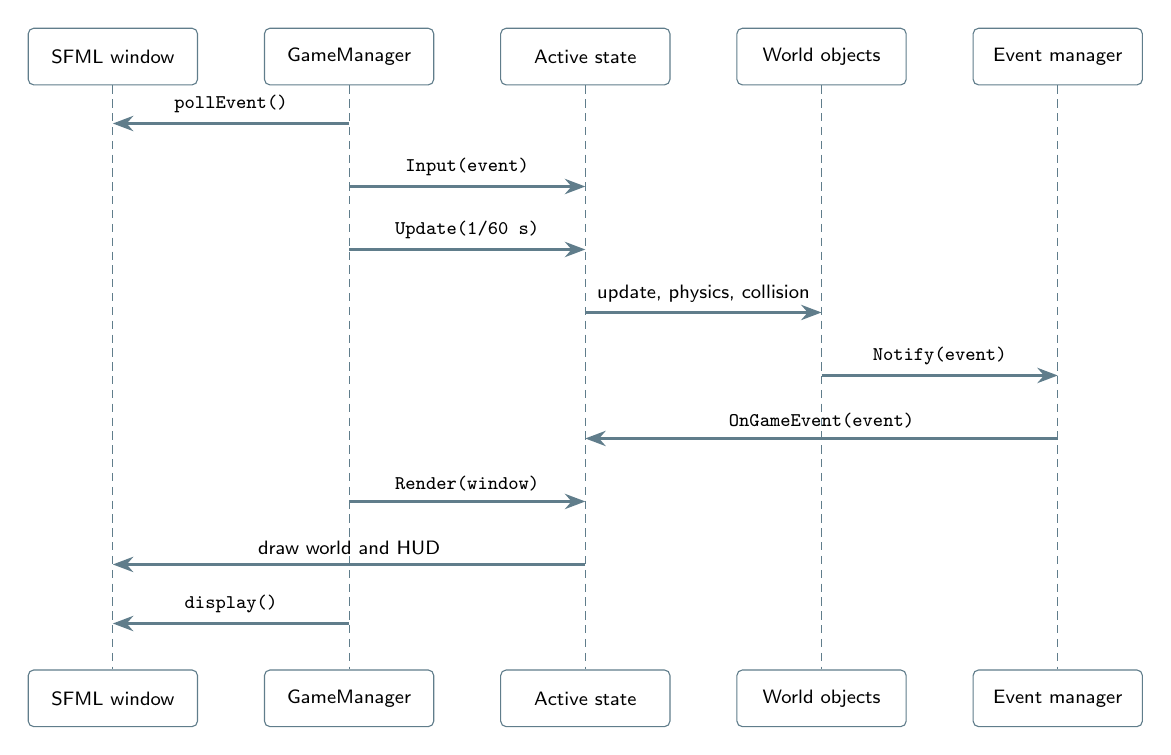
\begin{tikzpicture}[font=\sffamily\scriptsize]
        \tikzset{participant/.style={
            draw=gamegray,
            fill=white,
            rounded corners=2pt,
            minimum width=2.15cm,
            minimum height=0.72cm,
            align=center
        }}

        \node[participant] (windowTop) at (0,0) {SFML window};
        \node[participant] (managerTop) at (3,0) {GameManager};
        \node[participant] (stateTop) at (6,0) {Active state};
        \node[participant] (worldTop) at (9,0) {World objects};
        \node[participant] (eventTop) at (12,0) {Event manager};

        \node[participant] (windowBottom) at (0,-8.15) {SFML window};
        \node[participant] (managerBottom) at (3,-8.15) {GameManager};
        \node[participant] (stateBottom) at (6,-8.15) {Active state};
        \node[participant] (worldBottom) at (9,-8.15) {World objects};
        \node[participant] (eventBottom) at (12,-8.15) {Event manager};

        \draw[densely dashed,draw=gamegray]
            (windowTop.south) -- (windowBottom.north);
        \draw[densely dashed,draw=gamegray]
            (managerTop.south) -- (managerBottom.north);
        \draw[densely dashed,draw=gamegray]
            (stateTop.south) -- (stateBottom.north);
        \draw[densely dashed,draw=gamegray]
            (worldTop.south) -- (worldBottom.north);
        \draw[densely dashed,draw=gamegray]
            (eventTop.south) -- (eventBottom.north);

        \draw[architecturearrow] (3,-0.85) --
            node[above]{\texttt{pollEvent()}} (0,-0.85);
        \draw[architecturearrow] (3,-1.65) --
            node[above]{\texttt{Input(event)}} (6,-1.65);
        \draw[architecturearrow] (3,-2.45) --
            node[above]{\texttt{Update(1/60 s)}} (6,-2.45);
        \draw[architecturearrow] (6,-3.25) --
            node[above]{update, physics, collision} (9,-3.25);
        \draw[architecturearrow] (9,-4.05) --
            node[above]{\texttt{Notify(event)}} (12,-4.05);
        \draw[architecturearrow] (12,-4.85) --
            node[above]{\texttt{OnGameEvent(event)}} (6,-4.85);
        \draw[architecturearrow] (3,-5.65) --
            node[above]{\texttt{Render(window)}} (6,-5.65);
        \draw[architecturearrow] (6,-6.45) --
            node[above]{draw world and HUD} (0,-6.45);
        \draw[architecturearrow] (3,-7.20) --
            node[above]{\texttt{display()}} (0,-7.20);
    \end{tikzpicture}
    \caption{Representative input--update--event--render iteration.}
    \label{fig:main-loop-sequence}
\end{figure}

\section{Object-Oriented Design}

\subsection{Class Model}

Figure~\ref{fig:class-diagram} presents the principal ownership and dependency
relationships. The model deliberately omits small visual helpers and
short-lived value objects so that the boundaries governing the game loop and
the gameplay world remain visible. A solid blue arrow denotes exclusive
ownership or a value member, a dashed arrow denotes creation or use, and an
open triangular arrow denotes inheritance or interface implementation.

\begin{figure}[H]
    \centering
    \resizebox{\textwidth}{!}{%
    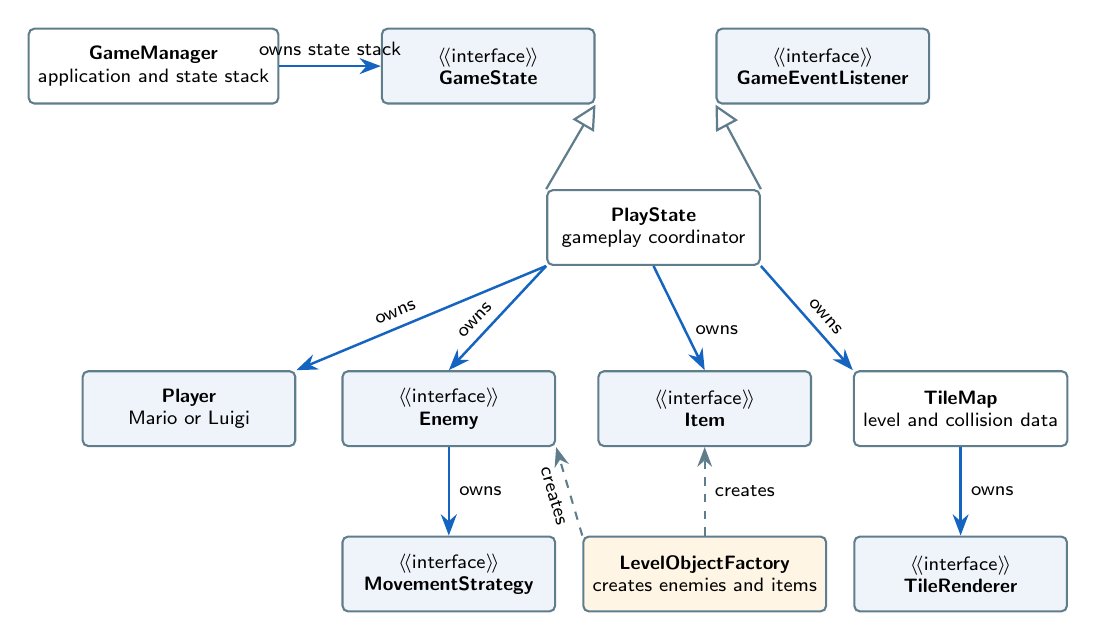
\begin{tikzpicture}[font=\sffamily\scriptsize]
        \tikzset{
            oopclass/.style={
                draw=gamegray,
                fill=white,
                rounded corners=2pt,
                line width=0.75pt,
                minimum width=2.7cm,
                minimum height=0.95cm,
                align=center
            },
            oopinterface/.style={
                oopclass,
                fill=marioblue!7
            },
            oopservice/.style={
                oopclass,
                fill=mariogold!12
            },
            oopinherit/.style={
                -{Triangle[open,length=3.1mm,width=3.1mm]},
                draw=gamegray,
                line width=0.8pt
            },
            oopowns/.style={
                -{Stealth[length=2.7mm]},
                draw=marioblue,
                line width=0.9pt
            },
            oopuses/.style={
                -{Stealth[length=2.5mm]},
                draw=gamegray,
                dashed,
                line width=0.75pt
            }
        }

        \node[oopclass] (manager) at (0,0)
            {\textbf{GameManager}\\application and state stack};
        \node[oopinterface] (state) at (4.25,0)
            {$\langle\!\langle$interface$\rangle\!\rangle$\\\textbf{GameState}};
        \node[oopinterface] (listener) at (8.5,0)
            {$\langle\!\langle$interface$\rangle\!\rangle$\\\textbf{GameEventListener}};

        \node[oopclass] (play) at (6.35,-2.05)
            {\textbf{PlayState}\\gameplay coordinator};

        \node[oopinterface] (player) at (0.45,-4.35)
            {\textbf{Player}\\Mario or Luigi};
        \node[oopinterface] (enemy) at (3.75,-4.35)
            {$\langle\!\langle$interface$\rangle\!\rangle$\\\textbf{Enemy}};
        \node[oopinterface] (item) at (7.0,-4.35)
            {$\langle\!\langle$interface$\rangle\!\rangle$\\\textbf{Item}};
        \node[oopclass] (tilemap) at (10.25,-4.35)
            {\textbf{TileMap}\\level and collision data};

        \node[oopinterface] (strategy) at (3.75,-6.45)
            {$\langle\!\langle$interface$\rangle\!\rangle$\\\textbf{MovementStrategy}};
        \node[oopservice] (factory) at (7.0,-6.45)
            {\textbf{LevelObjectFactory}\\creates enemies and items};
        \node[oopinterface] (renderer) at (10.25,-6.45)
            {$\langle\!\langle$interface$\rangle\!\rangle$\\\textbf{TileRenderer}};

        \draw[oopowns] (manager.east) --
            node[above]{owns state stack} (state.west);
        \draw[oopinherit] (play.north west) -- (state.south east);
        \draw[oopinherit] (play.north east) -- (listener.south west);

        \draw[oopowns] (play.south west) --
            node[above,sloped,pos=0.58]{owns} (player.north east);
        \draw[oopowns] (play.south west) --
            node[above,sloped,pos=0.62]{owns} (enemy.north);
        \draw[oopowns] (play.south) --
            node[right,pos=0.62]{owns} (item.north);
        \draw[oopowns] (play.south east) --
            node[above,sloped,pos=0.58]{owns} (tilemap.north west);

        \draw[oopowns] (enemy.south) --
            node[right]{owns} (strategy.north);
        \draw[oopowns] (tilemap.south) --
            node[right]{owns} (renderer.north);

        \draw[oopuses] (factory.north west) --
            node[below,sloped]{creates} (enemy.south east);
        \draw[oopuses] (factory.north) --
            node[right]{creates} (item.south);
    \end{tikzpicture}}
    \caption{Core class relationships, ownership, and dependencies.}
    \label{fig:class-diagram}
\end{figure}

The main runtime interfaces are expanded in
Figure~\ref{fig:oop-hierarchies}. Each hierarchy models a genuine ``is-a''
relationship, whereas variable behavior such as enemy movement and tile
rendering is supplied through composition.

\begin{figure}[H]
    \centering
    \resizebox{\textwidth}{!}{%
    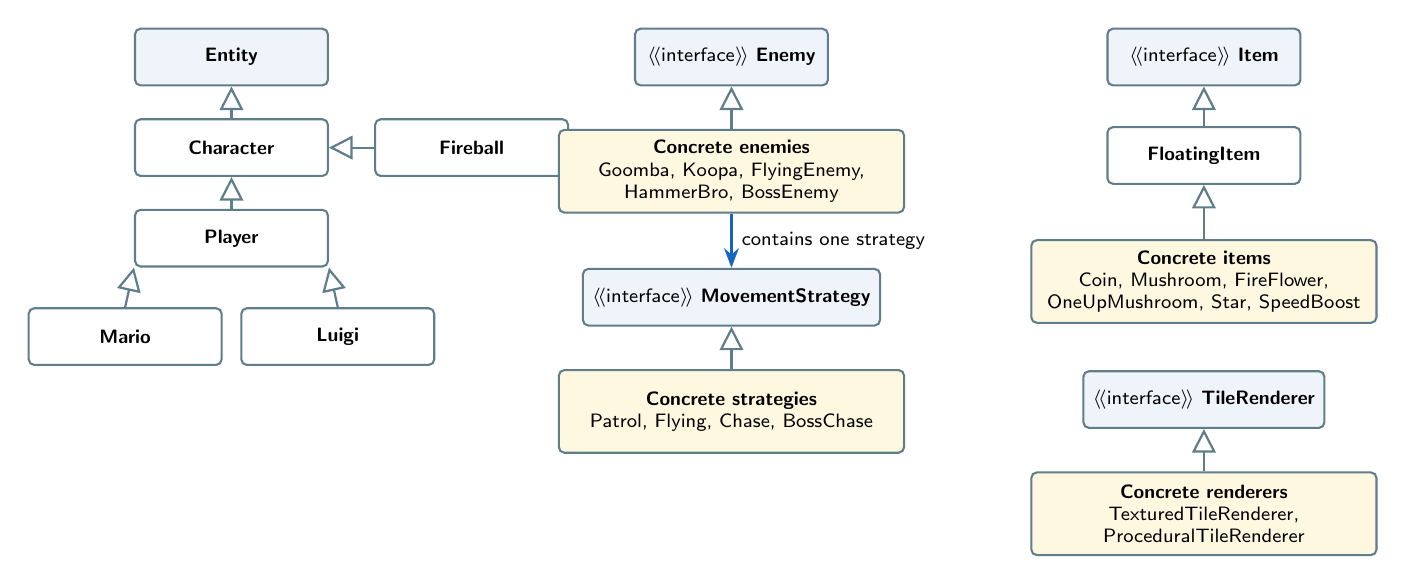
\begin{tikzpicture}[font=\sffamily\scriptsize]
        \tikzset{
            family/.style={
                draw=gamegray,
                fill=white,
                rounded corners=2pt,
                line width=0.75pt,
                minimum width=2.45cm,
                minimum height=0.72cm,
                align=center
            },
            familyinterface/.style={family,fill=marioblue!7},
            familygroup/.style={
                family,
                fill=gamelight,
                text width=4.15cm,
                minimum height=1.05cm
            },
            familyinherit/.style={
                -{Triangle[open,length=3mm,width=3mm]},
                draw=gamegray,
                line width=0.8pt
            },
            familyowns/.style={
                -{Stealth[length=2.5mm]},
                draw=marioblue,
                line width=0.8pt
            }
        }

        \node[familyinterface] (entity) at (0,0) {\textbf{Entity}};
        \node[family] (character) at (0,-1.15) {\textbf{Character}};
        \node[family] (playerbase) at (0,-2.30) {\textbf{Player}};
        \node[family] (mario) at (-1.35,-3.55) {\textbf{Mario}};
        \node[family] (luigi) at (1.35,-3.55) {\textbf{Luigi}};
        \node[family] (fireball) at (3.05,-1.15) {\textbf{Fireball}};

        \draw[familyinherit] (character.north) -- (entity.south);
        \draw[familyinherit] (playerbase.north) -- (character.south);
        \draw[familyinherit] (mario.north) -- (playerbase.south west);
        \draw[familyinherit] (luigi.north) -- (playerbase.south east);
        \draw[familyinherit] (fireball.west) -- (character.east);

        \node[familyinterface] (enemybase) at (6.35,0)
            {$\langle\!\langle$interface$\rangle\!\rangle$ \textbf{Enemy}};
        \node[familygroup] (enemytypes) at (6.35,-1.45)
            {\textbf{Concrete enemies}\\Goomba, Koopa, FlyingEnemy,\\HammerBro, BossEnemy};
        \node[familyinterface] (movementbase) at (6.35,-3.05)
            {$\langle\!\langle$interface$\rangle\!\rangle$ \textbf{MovementStrategy}};
        \node[familygroup] (movementtypes) at (6.35,-4.50)
            {\textbf{Concrete strategies}\\Patrol, Flying, Chase, BossChase};

        \draw[familyinherit] (enemytypes.north) -- (enemybase.south);
        \draw[familyinherit] (movementtypes.north) -- (movementbase.south);
        \draw[familyowns] (enemytypes.south) --
            node[right]{contains one strategy} (movementbase.north);

        \node[familyinterface] (itembase) at (12.35,0)
            {$\langle\!\langle$interface$\rangle\!\rangle$ \textbf{Item}};
        \node[family] (floating) at (12.35,-1.25)
            {\textbf{FloatingItem}};
        \node[familygroup] (itemtypes) at (12.35,-2.85)
            {\textbf{Concrete items}\\Coin, Mushroom, FireFlower,\\OneUpMushroom, Star, SpeedBoost};
        \node[familyinterface] (renderbase) at (12.35,-4.35)
            {$\langle\!\langle$interface$\rangle\!\rangle$ \textbf{TileRenderer}};
        \node[familygroup] (rendertypes) at (12.35,-5.80)
            {\textbf{Concrete renderers}\\TexturedTileRenderer,\\ProceduralTileRenderer};

        \draw[familyinherit] (floating.north) -- (itembase.south);
        \draw[familyinherit] (itemtypes.north) -- (floating.south);
        \draw[familyinherit] (rendertypes.north) -- (renderbase.south);
    \end{tikzpicture}}
    \caption{Principal inheritance and implementation hierarchies.}
    \label{fig:oop-hierarchies}
\end{figure}

\subsection{Core Class Responsibilities}

{\small
\begin{longtable}{@{}>{\raggedright\arraybackslash}p{4.10cm}
                        >{\raggedright\arraybackslash}p{5.80cm}
                        >{\raggedright\arraybackslash}p{4.65cm}@{}}
    \caption{Responsibilities of core classes.}\label{tab:classes}\\
    \toprule
    \textbf{Class/interface} & \textbf{Responsibility} &
    \textbf{Important collaborators} \\
    \midrule
    \endfirsthead
    \toprule
    \textbf{Class/interface} & \textbf{Responsibility} &
    \textbf{Important collaborators} \\
    \midrule
    \endhead
    \texttt{GameManager} & Owns the SFML window and the stack of application
    states; performs fixed-step input, update, and render dispatch; applies
    deferred state transitions safely. & \texttt{GameState},
    \texttt{SettingsManager}, audio and resource services. \\
    \texttt{GameState} and concrete states & Define a common screen lifecycle
    through \texttt{Input}, \texttt{Update}, and \texttt{Render}; each concrete
    state implements one menu, gameplay, pause, failure, or completion flow. &
    \texttt{GameManager}; \texttt{PlayState}, \texttt{PauseState}, menu and
    selection states. \\
    \texttt{Entity}/\texttt{Character} & Store the shared transform, velocity,
    dimensions, active state, facing direction, and collision callback used by
    movable world objects. & \texttt{Player}, \texttt{Fireball},
    \texttt{TileMap}. \\
    \texttt{Player}, \texttt{Mario}, \texttt{Luigi} & Implement buffered
    movement and jumping, power-up and animation states, damage transitions,
    character-specific speed, jump power, sprites, and rendering. &
    \texttt{PlayState}, \texttt{TileMap}, items, HUD, camera. \\
    \texttt{Enemy}/\allowbreak\texttt{MovementStrategy} & Provide the common enemy
    update, render, collision, damage, and activation contract while delegating
    reusable movement algorithms to injected strategies. & Concrete enemies,
    strategy classes, \texttt{EnemyFactory}, \texttt{PlayState}. \\
    \texttt{Item}/\allowbreak\texttt{FloatingItem} & Define collection and effect
    reporting; centralize bobbing, spawn animation, and collected state while
    concrete items supply visuals and an \texttt{ItemEffect}. & Concrete item
    classes, \texttt{ItemFactory}, \texttt{PlayState}, event system. \\
    \texttt{TileMap}/\allowbreak\texttt{TileRenderer} & Own parsed level data and tile
    geometry, resolve character--terrain collisions, update breakable blocks,
    and render through a textured or procedural backend. & \texttt{LevelLoader},
    \texttt{LevelData}, \texttt{Character}, renderer implementations. \\
    \texttt{LevelObjectFactory} & Convert neutral map spawn symbols into
    owning pointers to the correct enemy or item type and supply appropriate
    movement strategies. & \texttt{EnemyFactory}, \texttt{ItemFactory},
    \texttt{TileMap}, \texttt{PlayState}. \\
    Event interfaces and manager & Publish typed gameplay events and notify
    subscribed listeners without requiring producers to know score, audio, HUD,
    or projectile-handling details. & \texttt{GameEvent},
    \texttt{GameEventListener}, \texttt{PlayState}, enemies and items. \\
    Resource, audio, and persistence services & Cache expensive SFML assets,
    control music/effects, validate save fields, and expose save/load operations
    at infrastructure boundaries. & States, UI components, renderers,
    \texttt{SaveData}. \\
    \bottomrule
\end{longtable}
}

\subsection{Encapsulation}

Mutable game state is kept inside the class responsible for maintaining its
invariants. For example, \texttt{Player.hpp} keeps movement timers, animation
frames, power-up state, transformation flags, death state, and knockback data
as protected members. Other systems do not edit these variables directly.
They request domain operations such as \texttt{jump()},
\texttt{getMushroom()}, \texttt{up2Fire()}, \texttt{shrinkPlayer()}, or
\texttt{die()}, while read-only queries such as \texttt{isSuper()} and
\texttt{powerUpState()} expose only the information needed by
\texttt{PlayState}. These operations keep related changes synchronized; for
example, changing a power-up also recalculates jump power and resets mutually
exclusive transformation flags.

The item subsystem provides a second clear example. \texttt{FloatingItem}
keeps its base position, floating phase, spawn progress, and collected flag
private. Its public \texttt{Update}, \texttt{Collect}, and
\texttt{IsCollected} functions are marked \texttt{final}, so every item follows
the same lifecycle. Derived items can only implement the protected visual hooks
\texttt{SetVisualPosition} and \texttt{Animate}, which prevents them from
accidentally bypassing collection or spawn rules.

Encapsulation is also applied at the persistence boundary. Before writing,
\texttt{SaveManager.cpp} checks the version, level range, score, lives,
character, power-up value, coordinates, timer, and coin count. The load path
parses into a temporary \texttt{SaveData}, validates it, and returns
\texttt{std::optional<SaveData>}; therefore malformed external text is not
allowed to become active gameplay state.

\subsection{Inheritance}

The player branch begins with the abstract \texttt{Entity} contract for named,
updatable, renderable objects with a transform. \texttt{Character} extends it
with facing, grounded/roof state, and collision resolution;
\texttt{Player} then adds input, platforming mechanics, power-ups, and player
animation state. \texttt{Mario} and \texttt{Luigi} are concrete players because
each satisfies the complete player contract but supplies different movement
parameters and sprite handling. \texttt{Fireball} also derives from
\texttt{Character}, reusing transform and collision-facing behavior without
pretending to be a player.

Independent interface hierarchies model other substitutable families.
\texttt{Enemy} is implemented by \texttt{Goomba}, \texttt{Koopa},
\texttt{FlyingEnemy}, \texttt{HammerBro}, and \texttt{BossEnemy};
\texttt{Item} is refined by \texttt{FloatingItem} and its six concrete item
types; \texttt{GameState} is implemented by all application screens; and
\texttt{TileRenderer} is implemented by the textured and procedural renderers.
All polymorphic bases have virtual destructors, so deleting an object through
a base pointer invokes the complete derived destructor.

Inheritance is limited to stable semantic contracts. Enemy movement is not
encoded through additional enemy subclasses: a concrete enemy instead owns a
\texttt{MovementStrategy}. Likewise, \texttt{TileMap} owns a
\texttt{TileRenderer} rather than inheriting rendering behavior. Composition is
used in these cases because the behavior varies independently from the object
that uses it and can be selected during construction or level loading.

\subsection{Polymorphism}

Runtime polymorphism is used on the main execution paths rather than only in
the class declarations. \texttt{GameManager} stores
\texttt{std::unique\_ptr<GameState>} objects and dispatches input, fixed-step
updates, rendering, pause, and resume through the base interface. It therefore
does not need a screen-type switch when the active state changes from a menu to
gameplay or when \texttt{PauseState} is pushed as an overlay.

Similarly, \texttt{PlayState} owns heterogeneous enemies and items in
\texttt{std::vector<std::unique\_ptr<Enemy>>} and
\texttt{std::vector<std::unique\_ptr<Item>>}. The update and render loops call
\texttt{Update}, \texttt{Render}, \texttt{GetBounds}, and activation or
collection queries uniformly. The concrete response remains type-specific: a
boss can absorb several hits, a Koopa can become a movable shell, and each item
returns a different \texttt{ItemEffect}. Inactive objects are removed with the
erase--remove idiom; destruction is safe because both interfaces have virtual
destructors.

Two further dispatch points reduce conditional logic. Every enemy invokes its
owned \texttt{MovementStrategy} through the same virtual \texttt{Update}
operation, allowing patrol, vertical flight, chase, or boss chase behavior to
be selected by the factory. \texttt{TileMap} similarly delegates geometry and
drawing to a \texttt{TileRenderer}; the same map code can use
\texttt{TexturedTileRenderer} when the tileset loads or
\texttt{ProceduralTileRenderer} as a fallback.

\subsection{Abstraction}

The principal abstractions separate policy from implementation detail:

\begin{itemize}
    \item \texttt{GameState} lets the application loop operate on a screen
          lifecycle without knowing the controls, widgets, or transition rules
          of an individual screen.
    \item \texttt{Enemy}, \texttt{Item}, and \texttt{ItemEffect} let gameplay
          collision code work with capabilities and effects rather than sprite
          classes. Creation details are hidden behind
          \texttt{LevelObjectFactory}, which translates parsed map symbols into
          owning base pointers.
    \item \texttt{MovementStrategy} hides the algorithm used to move an enemy,
          while \texttt{TileRenderer} hides whether tile geometry is textured
          or procedurally colored.
    \item The \texttt{Character::CollisionResolver} callback decouples player
          motion from a concrete level class. \texttt{PlayState} injects a
          resolver that delegates to \texttt{TileMap}, so the character code
          needs no map-format or tile-query knowledge.
    \item \texttt{ResourceManager} exposes textures, fonts, and sound buffers
          by path while hiding caching and load failure handling;
          \texttt{AudioManager} exposes semantic effects rather than requiring
          states to manage SFML sound channels. \texttt{SaveManager} and
          \texttt{LoadManager} similarly hide the plain-text file format behind
          validated operations on \texttt{SaveData}.
\end{itemize}

These boundaries keep SFML objects and file-format decisions near the modules
that own them. Higher-level gameplay code depends mainly on contracts and
domain data, which limits the number of classes affected when a renderer,
enemy behavior, menu screen, or persistence implementation changes.

\subsection{Memory and Resource Ownership}

Ownership follows RAII and is visible in member types. Objects with one clear
owner use \texttt{std::unique\_ptr}: the manager owns its states;
\texttt{PlayState} owns the selected player, enemies, items, projectiles, and
menu button; enemies own their movement strategies; \texttt{TileMap} owns its
renderer; and \texttt{Button} owns its command and optional nine-slice visual.
Factories return \texttt{unique\_ptr} values, so ownership is transferred with
\texttt{std::move} and no manual \texttt{delete} is required.

Small records and tightly coupled components are stored by value. Examples
include \texttt{SaveData}, \texttt{LevelData}, \texttt{ItemEffect},
\texttt{TileMap}, \texttt{GameHud}, \texttt{PlayerCamera}, vertex arrays, and
SFML shapes. References are used for temporary non-owning access, such as the
render window passed to \texttt{Render}, the \texttt{Character\&} received by
collision resolution, and the constant resource references returned by
\texttt{ResourceManager}. The collision callback captures \texttt{PlayState}
only while the owned player exists. The raw \texttt{Koopa*} stored as
\texttt{m\_heldShell} is also explicitly non-owning; removal code clears it
before the corresponding \texttt{unique\_ptr<Enemy>} is erased.

Shared ownership is reserved for SFML textures whose lifetime must outlast
sprites stored in copied or movable background records. Background layers,
cloud rendering, parallax backgrounds, and cracked-block visuals use
\texttt{std::shared\_ptr<sf::Texture>} for that purpose. General cached assets
do not require shared ownership: \texttt{ResourceManager} keeps one
\texttt{unique\_ptr} per path and lends stable constant references to clients.
At shutdown, the state stack is cleared first, audio is shut down, and the
resource caches are cleared. Container destruction and smart-pointer
destructors then release derived objects and SFML resources automatically,
reducing both leaks and dangling-resource references.

\section{Design Patterns}

The five patterns evaluated against the project requirement are Factory,
Singleton, Observer, State, and Strategy. They are used on active execution
paths and solve separate creation, lifetime, notification, mode-management,
and algorithm-selection problems. Pattern names and roles follow the standard
object-oriented terminology summarized in Reference~2. Command and Template
Method also appear in
the implementation and are documented in
Section~\ref{subsec:supporting-patterns}, but they are treated as supporting
patterns rather than substitutes for the five primary patterns.

\subsection{Pattern Summary}

\begin{table}[H]
    \centering
    \caption{Summary of design patterns used in the game.}
    \label{tab:pattern-summary}
    {\small
    \begin{tabularx}{\textwidth}{@{}
        >{\raggedright\arraybackslash}p{2.7cm}
        >{\raggedright\arraybackslash}X
        >{\raggedright\arraybackslash}X
        >{\raggedright\arraybackslash}p{3.1cm}@{}}
        \toprule
        \textbf{Pattern} & \textbf{Problem solved} &
        \textbf{Main participants} & \textbf{Evidence} \\
        \midrule
        Factory (Simple Factory) & Convert level symbols into correctly
        configured enemies and items. & \texttt{LevelObjectFactory},
        \texttt{EnemyFactory}, \texttt{ItemFactory}, product interfaces. &
        Factory source files; Figure~\ref{fig:pattern-factory}. \\
        Singleton & Maintain one application-wide owner for the window, audio,
        cached assets, and event registry. & \texttt{GameManager},
        \texttt{AudioManager}, \texttt{ResourceManager},
        \texttt{GameEventManager}. & Manager headers/sources;
        Figure~\ref{fig:pattern-singleton}. \\
        Observer & Broadcast typed gameplay events without coupling producers
        to score, HUD, audio, or projectile handling. &
        \texttt{GameEventManager}, \texttt{GameEventListener},
        \texttt{GameEvent}, \texttt{PlayState}. & Event sources and
        \texttt{PlayState.cpp}; Figure~\ref{fig:pattern-observer}. \\
        State & Give every screen an independent input/update/render lifecycle
        and support push, pop, change, and overlay behavior. &
        \texttt{GameManager}, \texttt{GameState}, concrete state classes. &
        \texttt{GameManager.cpp}; Figure~\ref{fig:pattern-state}. \\
        Strategy & Select enemy movement independently from enemy type. &
        \texttt{Enemy}, \texttt{MovementStrategy}, concrete strategies,
        \texttt{EnemyFactory}. & Strategy/enemy sources;
        Figure~\ref{fig:pattern-strategy}. \\
        \bottomrule
    \end{tabularx}
    }
\end{table}

\subsection{Pattern 1: Factory}

\subsubsection{Problem and Intent}

Level files describe objects with compact symbols instead of C++ class names.
For example, \texttt{G}, \texttt{K}, and \texttt{E} identify enemy families,
whereas \texttt{C}, \texttt{M}, and \texttt{F} identify items. Constructing all
concrete classes inside \texttt{PlayState} would make the gameplay coordinator
depend on every constructor, sprite size, speed, patrol boundary, and movement
strategy. The Factory pattern moves that variable construction policy to a
dedicated creation boundary.

The submitted implementation is specifically a \emph{Simple Factory}
variant, not the GoF Factory Method: \texttt{EnemyFactory::Create} and
\texttt{ItemFactory::Create} are static selection functions, and no creator
subclass overrides a virtual factory operation. This naming matches the course
requirement's broader ``Factory Pattern'' category while accurately describing
the code.

\subsubsection{Structure and Participants}

\texttt{PlayState} is the client. It receives neutral
\texttt{LevelSpawnRequest} records from the loaded \texttt{LevelData} and asks
\texttt{LevelObjectFactory} to create an object. The latter is a narrow facade
that delegates to \texttt{EnemyFactory} or \texttt{ItemFactory}. The abstract
products are \texttt{Enemy} and \texttt{Item}; their concrete products include
the five enemy classes and six item classes. Both factory branches return
\texttt{std::unique\_ptr} to make ownership transfer explicit.

\begin{figure}[H]
    \centering
    \resizebox{0.98\textwidth}{!}{%
    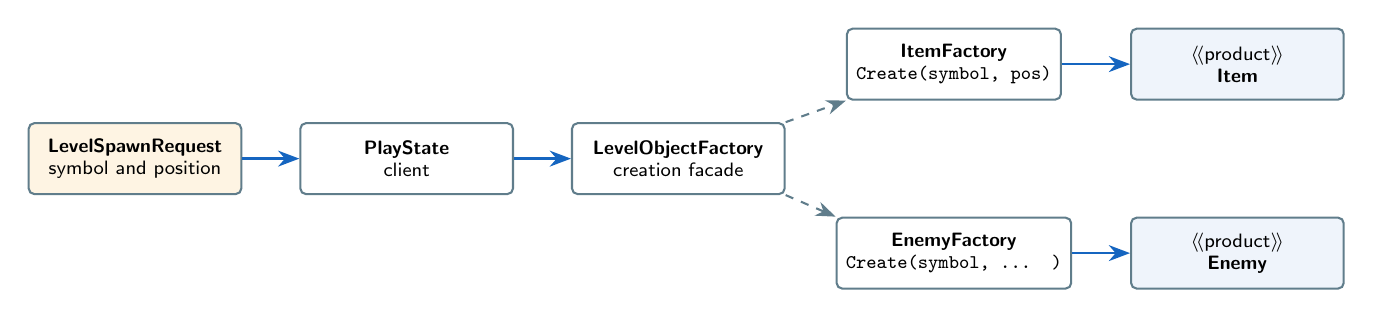
\begin{tikzpicture}
        \node[patternhighlight] (request) at (0,0)
            {\textbf{LevelSpawnRequest}\\symbol and position};
        \node[patternnode] (client) at (3.45,0)
            {\textbf{PlayState}\\client};
        \node[patternnode] (facade) at (6.9,0)
            {\textbf{LevelObjectFactory}\\creation facade};
        \node[patternnode] (itemfactory) at (10.4,1.2)
            {\textbf{ItemFactory}\\\texttt{Create(symbol, pos)}};
        \node[patternnode] (enemyfactory) at (10.4,-1.2)
            {\textbf{EnemyFactory}\\\texttt{Create(symbol, ... )}};
        \node[patterninterface] (itemproduct) at (14.0,1.2)
            {$\langle\!\langle$product$\rangle\!\rangle$\\\textbf{Item}};
        \node[patterninterface] (enemyproduct) at (14.0,-1.2)
            {$\langle\!\langle$product$\rangle\!\rangle$\\\textbf{Enemy}};

        \draw[patternarrow] (request.east) -- (client.west);
        \draw[patternarrow] (client.east) -- (facade.west);
        \draw[patternuses] (facade.north east) -- (itemfactory.south west);
        \draw[patternuses] (facade.south east) -- (enemyfactory.north west);
        \draw[patternarrow] (itemfactory.east) -- (itemproduct.west);
        \draw[patternarrow] (enemyfactory.east) -- (enemyproduct.west);
    \end{tikzpicture}}
    \caption{Factory structure for level-defined enemies and items.}
    \label{fig:pattern-factory}
\end{figure}

\subsubsection{Implementation Evidence}

The representative selection below is abridged from
\texttt{EnemyFactory.cpp}, lines 84--175. The complete function also computes
safe horizontal movement limits from \texttt{TileMap}; item selection appears
in \texttt{ItemFactory.cpp}, lines 12--55, and facade delegation appears in
\texttt{LevelObjectFactory.cpp}, lines 7--33.

\begin{lstlisting}[style=gamecode,basicstyle=\ttfamily\scriptsize,caption={Abridged enemy factory selection and strategy injection.}]
switch (symbol) {
case 'G':
    return std::make_unique<Goomba>(
        position, 70.f,
        std::make_unique<ChaseStrategy>(
            minimumX, maximumX, 280.f, true));

case 'E':
    return std::make_unique<FlyingEnemy>(
        position, 80.f,
        std::make_unique<FlyingStrategy>(
            std::max(0.f, position.y - tileSize * 3.f),
            position.y + tileSize * 4.f));

case 'Z':
    return std::make_unique<BossEnemy>(
        sf::Vector2f(position.x + tileSize * 0.5f,
                     position.y + tileSize),
        25.f,
        std::make_unique<BossChaseStrategy>(minimumX, maximumX));

default:
    throw std::invalid_argument("Unsupported enemy map symbol");
}
\end{lstlisting}

When the loader encounters \texttt{G}, the client receives an owning
\texttt{Enemy} pointer whose dynamic type is \texttt{Goomba} and whose movement
dependency is a configured \texttt{ChaseStrategy}. The client neither names
that concrete type nor manages partial construction. This centralization makes
map parsing and gameplay code stable when constructor parameters change. The
trade-off is that adding a new symbol still requires modifying a centralized
\texttt{switch}; a registry or data-driven constructor table would be more
open-ended if the number of products became much larger.

\subsection{Pattern 2: Singleton}

\subsubsection{Problem and Intent}

Several services represent one application-wide resource: there must be one
window and state stack, one active music controller, one gameplay listener
registry, and one cache entry for each loaded asset path. Passing all four
services through every state, entity, and UI constructor would add substantial
plumbing, while accidentally duplicating them could create competing windows,
music streams, event registries, or SFML resources. The project therefore uses
Singleton for \texttt{GameManager}, \texttt{AudioManager},
\texttt{GameEventManager}, and \texttt{ResourceManager}.

\subsubsection{Structure and Participants}

\texttt{ResourceManager} is the clearest representative. It has a private
constructor, deleted copy operations, and a public \texttt{getInstance()}
access point returning a function-local static object. States, enemies, and UI
components are clients. The singleton owns maps of textures, fonts, and sound
buffers and lends stable constant references to the loaded resources.

\begin{figure}[H]
    \centering
    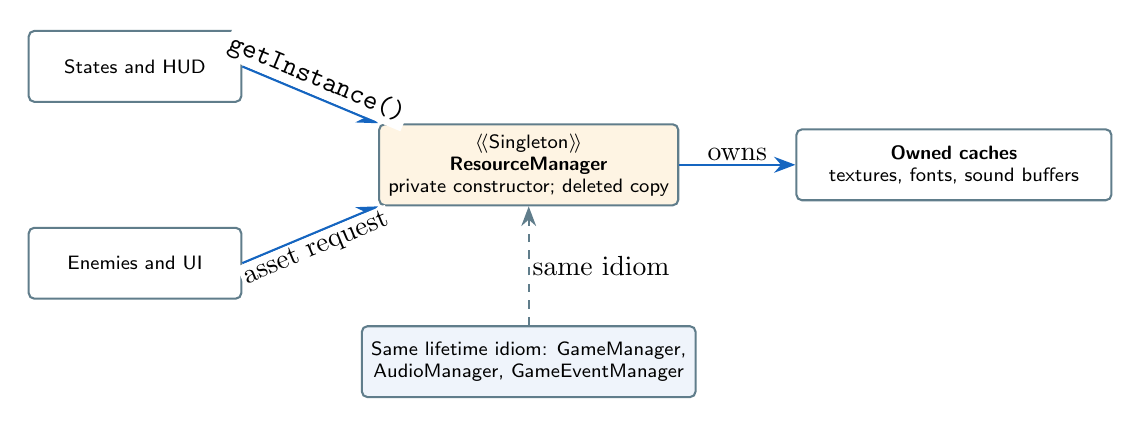
\begin{tikzpicture}
        \node[patternnode] (states) at (0,1.25)
            {States and HUD};
        \node[patternnode] (entities) at (0,-1.25)
            {Enemies and UI};
        \node[patternhighlight,minimum width=3.5cm] (singleton) at (5.0,0)
            {$\langle\!\langle$Singleton$\rangle\!\rangle$\\
             \textbf{ResourceManager}\\private constructor; deleted copy};
        \node[patternnode,minimum width=4.0cm] (cache) at (10.4,0)
            {\textbf{Owned caches}\\textures, fonts, sound buffers};
        \node[patterninterface,minimum width=4.1cm] (peers) at (5.0,-2.5)
            {Same lifetime idiom: GameManager,\\AudioManager, GameEventManager};

        \draw[patternarrow] (states.east) --
            node[above,sloped,fill=white,inner sep=1pt]
            {\texttt{getInstance()}} (singleton.north west);
        \draw[patternarrow] (entities.east) --
            node[below,sloped,fill=white,inner sep=1pt]{asset request}
            (singleton.south west);
        \draw[patternarrow] (singleton.east) --
            node[above,fill=white,inner sep=1pt]{owns} (cache.west);
        \draw[patternuses] (peers.north) --
            node[right,fill=white,inner sep=1pt]{same idiom} (singleton.south);
    \end{tikzpicture}
    \caption{Singleton access and ownership represented by ResourceManager.}
    \label{fig:pattern-singleton}
\end{figure}

\subsubsection{Implementation Evidence}

The instance and cache logic is implemented in the
\texttt{ResourceManager} header (lines 11--29) and source (lines 5--23). A real
client can be seen in the
\texttt{Goomba} constructor at \texttt{Goomba.cpp}, lines 25--27.

\begin{lstlisting}[style=gamecode,basicstyle=\ttfamily\scriptsize,caption={Singleton construction, copy prevention, and lazy cache access.}]
class ResourceManager {
public:
    static ResourceManager& getInstance();
    ResourceManager(const ResourceManager&) = delete;
    ResourceManager& operator=(const ResourceManager&) = delete;
private:
    ResourceManager() = default;
};

ResourceManager& ResourceManager::getInstance() {
    static ResourceManager instance;
    return instance;
}

const sf::Texture& ResourceManager::getTexture(const std::string& path) {
    const auto existing = m_textures.find(path);
    if (existing != m_textures.end()) return *existing->second;
    auto texture = std::make_unique<sf::Texture>();
    if (!texture->loadFromFile(path)) throw std::runtime_error(path);
    const sf::Texture& resource = *texture;
    m_textures.emplace(path, std::move(texture));
    return resource;
}
\end{lstlisting}

The function-local static is initialized on first access and destroyed at
program termination. C++ guarantees safe initialization of that local static,
but subsequent map and audio operations are not synchronized; this is
acceptable because the submitted game loads and uses services on its single
main thread. \texttt{GameManager::run} explicitly destroys states, shuts down
audio, and clears resource caches in that order. The pattern prevents duplicate
service instances and provides convenient access, but it introduces global
dependencies and makes isolated tests harder because clients cannot easily
substitute a fake service.

\subsection{Pattern 3: Observer}

\subsubsection{Problem and Intent}

Gameplay actions often have several consequences. Defeating an enemy changes
the score, plays a sound, and updates the status display; collecting an item
may change player state, lives, timers, and HUD data; a boss or Hammer Bro can
request a projectile without owning the projectile container. Direct calls
from every producer to all affected systems would create circular and
many-to-many dependencies. Observer replaces those calls with typed
\texttt{GameEvent} notifications.

\subsubsection{Structure and Participants}

\texttt{GameEventManager} is the publisher/subject and stores non-owning
\texttt{GameEventListener*} subscriptions. \texttt{GameEventListener} is the
observer interface, and \texttt{PlayState} is the concrete observer. Producers
include collision logic, \texttt{BossEnemy}, and \texttt{HammerBro}. The event
object carries an enumerated type, an integer value, and optional string data.

\begin{figure}[H]
    \centering
    \resizebox{0.98\textwidth}{!}{%
    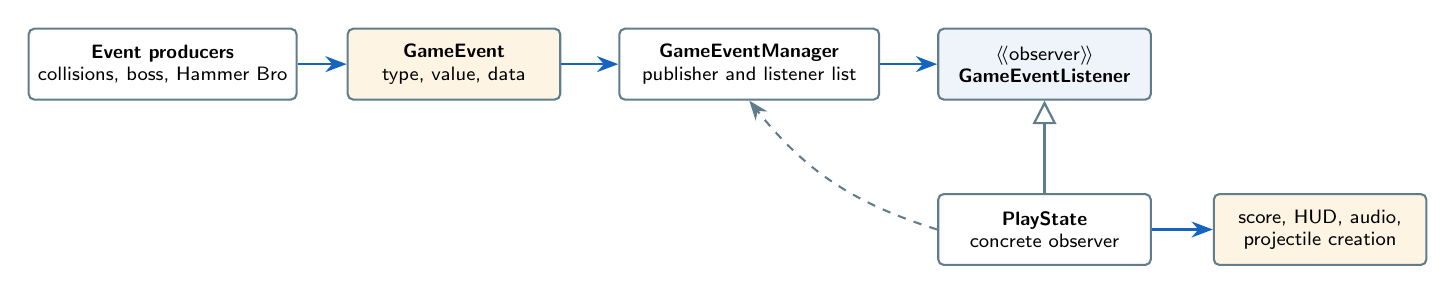
\begin{tikzpicture}
        \node[patternnode] (producer) at (0,0)
            {\textbf{Event producers}\\collisions, boss, Hammer Bro};
        \node[patternhighlight] (event) at (3.7,0)
            {\textbf{GameEvent}\\type, value, data};
        \node[patternnode,minimum width=3.3cm] (subject) at (7.45,0)
            {\textbf{GameEventManager}\\publisher and listener list};
        \node[patterninterface] (observer) at (11.2,0)
            {$\langle\!\langle$observer$\rangle\!\rangle$\\
             \textbf{GameEventListener}};
        \node[patternnode] (play) at (11.2,-2.1)
            {\textbf{PlayState}\\concrete observer};
        \node[patternhighlight] (effects) at (14.7,-2.1)
            {score, HUD, audio,\\projectile creation};

        \draw[patternarrow] (producer.east) -- (event.west);
        \draw[patternarrow] (event.east) -- (subject.west);
        \draw[patternarrow] (subject.east) -- (observer.west);
        \draw[patterninherit] (play.north) -- (observer.south);
        \draw[patternarrow] (play.east) -- (effects.west);
        \draw[patternuses] (play.west) to[bend left=17] (subject.south);
    \end{tikzpicture}}
    \caption{Observer relationships and synchronous notification flow.}
    \label{fig:pattern-observer}
\end{figure}

\subsubsection{Implementation Evidence}

Subscription and removal occur in \texttt{PlayState.cpp}, lines 96--101. The
publisher prevents duplicate subscriptions and implements broadcast in
\texttt{GameEventManager.cpp}, lines 11--58. The excerpt combines these two
parts with the boss publication at \texttt{BossEnemy.cpp}, lines 186--192.

\begin{lstlisting}[style=gamecode,basicstyle=\ttfamily\scriptsize,caption={Observer registration, publication, and notification.}]
// PlayState lifetime
GameEventManager::GetInstance().AddListener(this);
// PlayState::~PlayState()
GameEventManager::GetInstance().RemoveListener(this);

// BossEnemy::TakeDamage()
GameEventManager::GetInstance().Notify({
    GameEventType::EnemyDefeated,
    DEFEAT_SCORE,
    "Boss Defeated"
});

void GameEventManager::Notify(const GameEvent& event) {
    const auto listeners = m_listeners;
    for (GameEventListener* listener : listeners) {
        if (listener != nullptr) {
            listener->OnGameEvent(event);
        }
    }
}
\end{lstlisting}

Notification is synchronous: the producer completes the call only after each
current listener has handled the event. Copying the listener vector before
iteration prevents iterator invalidation if callbacks alter registration or
trigger nested events. \texttt{AddListener} rejects null and duplicate entries,
and \texttt{PlayState} unregisters in its destructor. The remaining trade-off
is the raw, non-owning listener list: every future listener must obey the same
unsubscription rule, and deeply nested synchronous events can make control flow
less obvious during debugging.

\subsection{Pattern 4: State}

\subsubsection{Problem and Intent}

The application contains menus, character and level selection, generated-level
configuration, gameplay, pause, options, about, game-over, and level-complete
screens. Each screen interprets input and renders differently. Encoding all of
these modes inside the main loop would produce a large conditional structure
and allow state-specific data to leak across transitions. State gives every
screen one implementation of a stable lifecycle contract.

\subsubsection{Structure and Participants}

\texttt{GameManager} is the context and owns
\texttt{std::unique\_ptr<GameState>} objects as a stack. \texttt{GameState} is
the state interface. The ten concrete states implement
\texttt{Input}/\texttt{Update}/\texttt{Render}; overlays additionally override
\texttt{isOverlay}. \texttt{pushState}, \texttt{popState}, and
\texttt{changeState} request transitions. A private pending-action queue
defers a transition requested while a state callback is being dispatched, so a
state is not destroyed in the middle of its own method.

\begin{figure}[H]
    \centering
    \resizebox{0.94\textwidth}{!}{%
    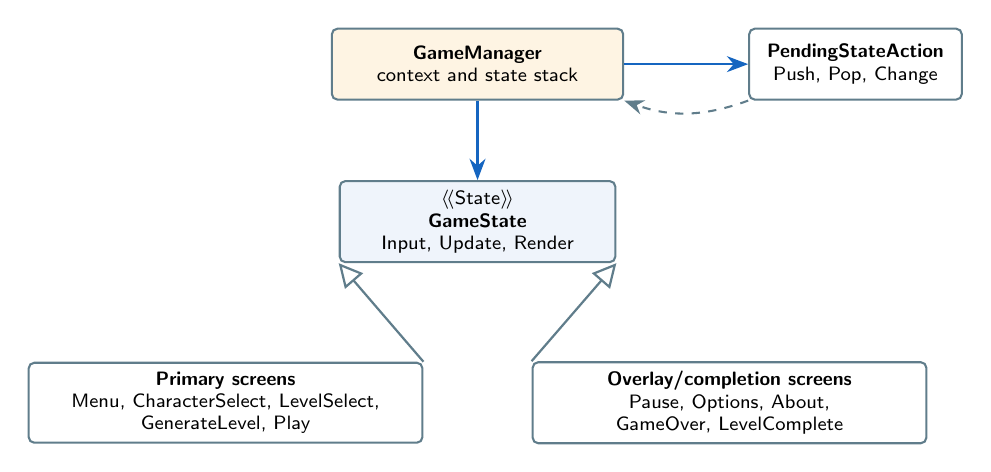
\begin{tikzpicture}
        \node[patternhighlight,minimum width=3.7cm] (context) at (5.7,0)
            {\textbf{GameManager}\\context and state stack};
        \node[patternnode] (pending) at (10.5,0)
            {\textbf{PendingStateAction}\\Push, Pop, Change};
        \node[patterninterface,minimum width=3.5cm] (state) at (5.7,-2.0)
            {$\langle\!\langle$State$\rangle\!\rangle$\\\textbf{GameState}\\
             Input, Update, Render};
        \node[patternnode,minimum width=5.0cm] (screens) at (2.5,-4.3)
            {\textbf{Primary screens}\\Menu, CharacterSelect, LevelSelect,\\
             GenerateLevel, Play};
        \node[patternnode,minimum width=5.0cm] (overlays) at (8.9,-4.3)
            {\textbf{Overlay/completion screens}\\Pause, Options, About,\\
             GameOver, LevelComplete};

        \draw[patternarrow] (context.south) -- (state.north);
        \draw[patternarrow] (context.east) -- (pending.west);
        \draw[patternuses] (pending.south west) to[bend left=20]
            (context.south east);
        \draw[patterninherit] (screens.north east) -- (state.south west);
        \draw[patterninherit] (overlays.north west) -- (state.south east);
    \end{tikzpicture}}
    \caption{State hierarchy, context ownership, and deferred transitions.}
    \label{fig:pattern-state}
\end{figure}

\subsubsection{Implementation Evidence}

The contract is declared in \texttt{GameState.hpp}, lines 5--15. Transition
requests and their guarded application are implemented in
\texttt{GameManager.cpp}, lines 22--87. A typical transition request is the
pause actions in \texttt{PlayState.cpp}, lines 48--50 and 275--278.

\begin{lstlisting}[style=gamecode,basicstyle=\ttfamily\scriptsize,caption={State contract and deferred transition request.}]
class GameState {
public:
    virtual ~GameState() = default;
    virtual void Input(const sf::Event& event) = 0;
    virtual void Update(sf::Time dt) = 0;
    virtual void Render(sf::RenderWindow& window) = 0;
    virtual bool isOverlay() const { return false; }
    virtual void onPause() {}
    virtual void onResume() {}
};

void GameManager::pushState(std::unique_ptr<GameState> state) {
    requestStateAction({StateActionType::Push, std::move(state)});
}

void GameManager::requestStateAction(PendingStateAction action) {
    if (m_isDispatchingState || m_isApplyingStateAction) {
        m_pendingStateActions.push_back(std::move(action));
        return;
    }
    applyStateAction(std::move(action));
    applyPendingStateActions();
}
\end{lstlisting}

Pressing the configured pause key causes \texttt{PlayState} to push a
\texttt{PauseState}. The manager invokes the gameplay state's pause hook, keeps the
gameplay state below the overlay, and dispatches new input and updates only to
the top state. Popping the overlay destroys it and resumes gameplay. Adding a
new screen therefore does not require modifying the main input/update/render
loop. The cost is a larger number of small classes and some transition
knowledge in concrete states; the singleton context also means transitions are
requested through a global access point.

\subsection{Pattern 5: Strategy}

\subsubsection{Problem and Intent}

Enemy appearance, combat rules, and movement do not vary along the same axis.
A Goomba and Koopa can both react to the player horizontally, a flying enemy
requires vertical oscillation, and the boss uses direct pursuit with a
dead-zone. Embedding each movement algorithm in every enemy would duplicate
boundary and direction logic. Strategy extracts movement into objects that can
be configured independently and injected when an enemy is created.

\subsubsection{Structure and Participants}

Each concrete enemy class is a context that stores one movement strategy.
Ownership is exclusive and represented by \texttt{std::unique\_ptr}.
\texttt{MovementStrategy} defines
\texttt{Update} and an optional player-position hook. Its concrete
implementations are \texttt{PatrolStrategy}, \texttt{FlyingStrategy},
\texttt{ChaseStrategy}, and \texttt{BossChaseStrategy}. The current factory
maps \texttt{G}, \texttt{K}, \texttt{H}, and \texttt{h} to
\texttt{ChaseStrategy}, \texttt{E} to \texttt{FlyingStrategy}, and
\texttt{Z} to \texttt{BossChaseStrategy}. \texttt{PatrolStrategy} remains an
implemented alternative but is not selected by the submitted symbol mapping.

\begin{figure}[H]
    \centering
    \resizebox{0.96\textwidth}{!}{%
    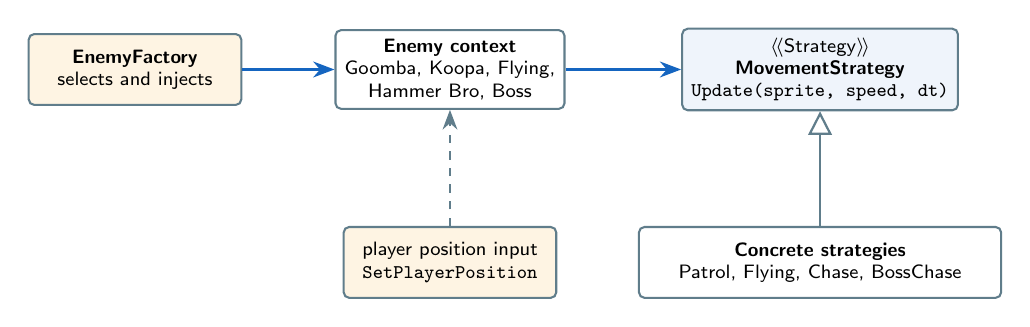
\begin{tikzpicture}
        \node[patternhighlight] (factory) at (0,0)
            {\textbf{EnemyFactory}\\selects and injects};
        \node[patternnode] (context) at (4.0,0)
            {\textbf{Enemy context}\\Goomba, Koopa, Flying,\\Hammer Bro, Boss};
        \node[patterninterface,minimum width=3.5cm] (strategy) at (8.7,0)
            {$\langle\!\langle$Strategy$\rangle\!\rangle$\\
             \textbf{MovementStrategy}\\\texttt{Update(sprite, speed, dt)}};
        \node[patternnode,minimum width=4.6cm] (concrete) at (8.7,-2.45)
            {\textbf{Concrete strategies}\\Patrol, Flying, Chase, BossChase};
        \node[patternhighlight] (playerpos) at (4.0,-2.45)
            {player position input\\\texttt{SetPlayerPosition}};

        \draw[patternarrow] (factory.east) -- (context.west);
        \draw[patternarrow] (context.east) -- (strategy.west);
        \draw[patterninherit] (concrete.north) -- (strategy.south);
        \draw[patternuses] (playerpos.north) -- (context.south);
    \end{tikzpicture}}
    \caption{Strategy selection, ownership, and movement delegation.}
    \label{fig:pattern-strategy}
\end{figure}

\subsubsection{Implementation Evidence}

The interface is declared in \texttt{MovementStrategy.hpp}, lines 5--16.
Constructor injection and delegation are visible in \texttt{Goomba.cpp}, lines
7--23 and 63--67, while the selection rules are in
\texttt{EnemyFactory.cpp}, lines 84--168.

\begin{lstlisting}[style=gamecode,basicstyle=\ttfamily\scriptsize,caption={Strategy ownership and delegation in Goomba.}]
Goomba::Goomba(
    sf::Vector2f position,
    float speed,
    std::unique_ptr<MovementStrategy> movementStrategy)
    : m_movementStrategy(std::move(movementStrategy)),
      m_speed(speed) {
    if (!m_movementStrategy) {
        throw std::invalid_argument(
            "Goomba requires a movement strategy.");
    }
}

void Goomba::Update(sf::Time timePerFrame) {
    // Animation and inactive/flung handling omitted.
    m_movementStrategy->Update(
        m_sprite, m_speed, timePerFrame);
}

void Goomba::SetPlayerPosition(sf::Vector2f pos) {
    m_movementStrategy->setPlayerPosition(pos);
}
\end{lstlisting}

For a \texttt{G} spawn, the factory constructs a \texttt{ChaseStrategy} with
terrain-derived movement bounds and a 280-pixel aggression radius, then moves
it into the new \texttt{Goomba}. \texttt{PlayState} supplies the player's
position through the base \texttt{Enemy} interface, and \texttt{Goomba}
forwards it to the strategy before delegating movement. The enemy class remains
focused on animation, damage, and rendering. The trade-offs are one heap-owned
strategy per enemy and an interface currently coupled to \texttt{sf::Sprite};
also, strategies are selected at construction and no public setter currently
supports swapping them later.

\subsection{Additional Supporting Patterns}
\label{subsec:supporting-patterns}

Two further patterns reinforce the primary design:

\begin{itemize}
    \item \textbf{Template Method:} \texttt{FloatingItem::Update} owns the
          invariant spawn and bobbing algorithm, then calls the protected hooks
          \texttt{SetVisualPosition} and \texttt{Animate}. The lifecycle
          methods \texttt{Update}, \texttt{Collect}, and
          \texttt{IsCollected} are \texttt{final}; concrete items vary visuals
          and effects without replacing the common lifecycle. Evidence appears
          in \texttt{FloatingItem.hpp}, lines 5--35, and
          \texttt{FloatingItem.cpp}, lines 15--49. This ensures consistent item
          behavior, at the cost of tying variation to inheritance and to a
          fixed update skeleton.
    \item \textbf{Command:} \texttt{Button} owns a
          \texttt{std::unique\_ptr<ICommand>} and invokes
          \texttt{execute()} after a click. \texttt{LambdaCommand},
          \texttt{PopStateCommand}, and \texttt{ExitGameCommand} encapsulate
          menu actions, so the reusable button class does not depend on game
          transitions. The interface is in \texttt{ICommand.hpp}; concrete
          commands are in \texttt{MenuCommands.hpp}. Invocation appears in
          \texttt{Button.cpp}, lines 80--92.
          The pattern supports dynamic menu construction. Its trade-off is
          that small lambda commands can make navigation logic less searchable
          than dedicated command classes.
\end{itemize}

\subsection{Pattern Interaction}

A boss encounter exercises all five primary patterns. While loading the
active \texttt{PlayState}, the Factory converts symbol \texttt{Z} into a
\texttt{BossEnemy} containing a \texttt{BossChaseStrategy}. The State context
later dispatches each fixed update to \texttt{PlayState}, which updates the
boss through the \texttt{Enemy} interface; the boss delegates movement to its
Strategy. When its health reaches zero, the boss publishes an
\texttt{EnemyDefeated} event. The Observer manager calls
\texttt{PlayState::OnGameEvent}, which changes score/status data and asks the
Singleton \texttt{AudioManager} to play the defeat effect.

\begin{figure}[H]
    \centering
    \resizebox{\textwidth}{!}{%
    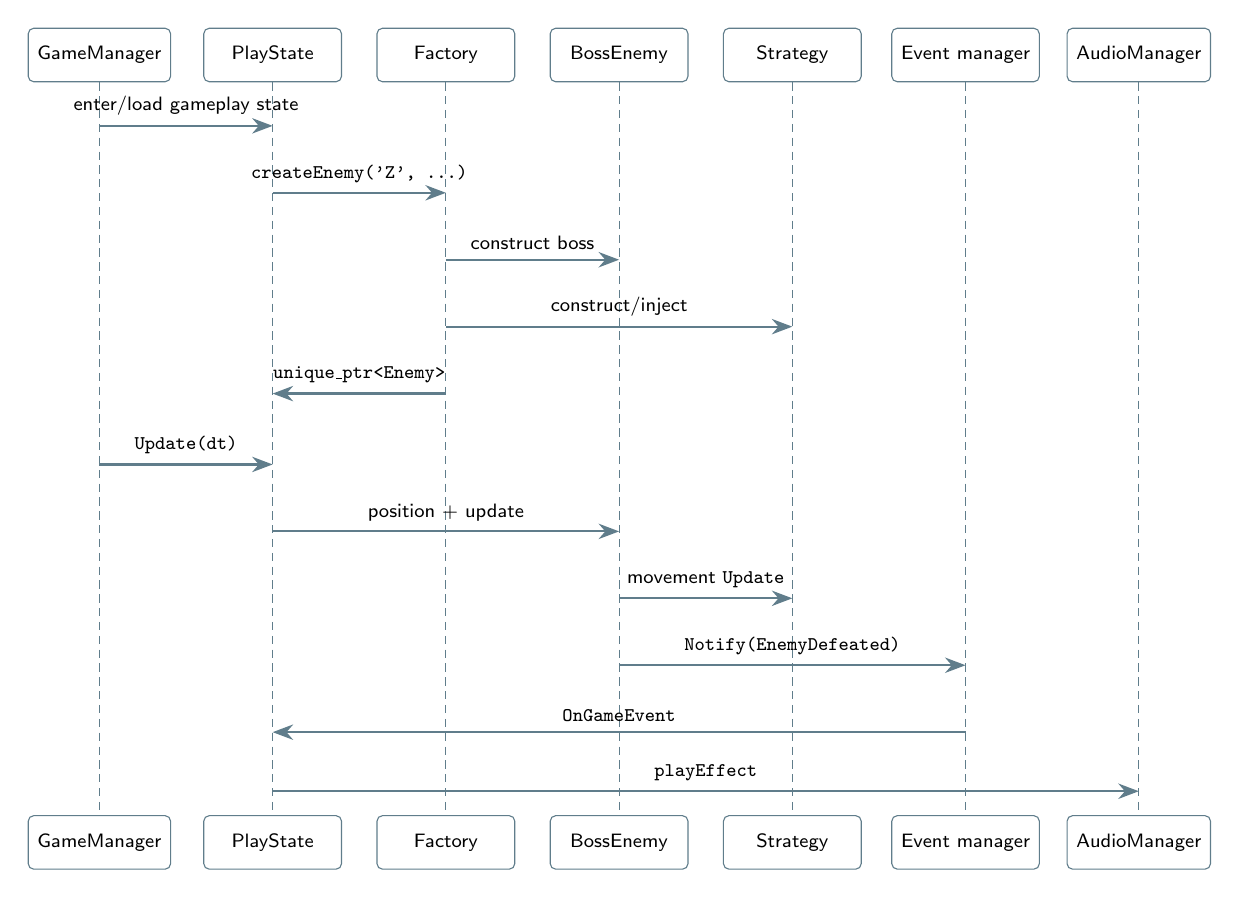
\begin{tikzpicture}[font=\sffamily\scriptsize]
        \tikzset{participant/.style={
            draw=gamegray,
            fill=white,
            rounded corners=2pt,
            minimum width=1.75cm,
            minimum height=0.68cm,
            align=center
        }}

        \node[participant] (managerTop) at (0,0) {GameManager};
        \node[participant] (playTop) at (2.2,0) {PlayState};
        \node[participant] (factoryTop) at (4.4,0) {Factory};
        \node[participant] (enemyTop) at (6.6,0) {BossEnemy};
        \node[participant] (strategyTop) at (8.8,0) {Strategy};
        \node[participant] (eventTop) at (11.0,0) {Event manager};
        \node[participant] (audioTop) at (13.2,0) {AudioManager};

        \node[participant] (managerBottom) at (0,-10.0) {GameManager};
        \node[participant] (playBottom) at (2.2,-10.0) {PlayState};
        \node[participant] (factoryBottom) at (4.4,-10.0) {Factory};
        \node[participant] (enemyBottom) at (6.6,-10.0) {BossEnemy};
        \node[participant] (strategyBottom) at (8.8,-10.0) {Strategy};
        \node[participant] (eventBottom) at (11.0,-10.0) {Event manager};
        \node[participant] (audioBottom) at (13.2,-10.0) {AudioManager};

        \draw[densely dashed,draw=gamegray]
            (managerTop.south) -- (managerBottom.north);
        \draw[densely dashed,draw=gamegray]
            (playTop.south) -- (playBottom.north);
        \draw[densely dashed,draw=gamegray]
            (factoryTop.south) -- (factoryBottom.north);
        \draw[densely dashed,draw=gamegray]
            (enemyTop.south) -- (enemyBottom.north);
        \draw[densely dashed,draw=gamegray]
            (strategyTop.south) -- (strategyBottom.north);
        \draw[densely dashed,draw=gamegray]
            (eventTop.south) -- (eventBottom.north);
        \draw[densely dashed,draw=gamegray]
            (audioTop.south) -- (audioBottom.north);

        \draw[architecturearrow] (0,-0.9) --
            node[above]{enter/load gameplay state} (2.2,-0.9);
        \draw[architecturearrow] (2.2,-1.75) --
            node[above]{\texttt{createEnemy('Z', ...)}} (4.4,-1.75);
        \draw[architecturearrow] (4.4,-2.6) --
            node[above]{construct boss} (6.6,-2.6);
        \draw[architecturearrow] (4.4,-3.45) --
            node[above]{construct/inject} (8.8,-3.45);
        \draw[architecturearrow] (4.4,-4.3) --
            node[above]{\texttt{unique\_ptr<Enemy>}} (2.2,-4.3);
        \draw[architecturearrow] (0,-5.2) --
            node[above]{\texttt{Update(dt)}} (2.2,-5.2);
        \draw[architecturearrow] (2.2,-6.05) --
            node[above]{position + update} (6.6,-6.05);
        \draw[architecturearrow] (6.6,-6.9) --
            node[above]{movement \texttt{Update}} (8.8,-6.9);
        \draw[architecturearrow] (6.6,-7.75) --
            node[above]{\texttt{Notify(EnemyDefeated)}} (11.0,-7.75);
        \draw[architecturearrow] (11.0,-8.6) --
            node[above]{\texttt{OnGameEvent}} (2.2,-8.6);
        \draw[architecturearrow] (2.2,-9.35) --
            node[above]{\texttt{playEffect}} (13.2,-9.35);
    \end{tikzpicture}}
    \caption{Interaction of Factory, State, Strategy, Observer, and Singleton
    during a boss encounter.}
    \label{fig:pattern-interaction}
\end{figure}

\section{Gameplay Implementation}

\subsection{Input, Movement, and Camera}

The main loop in \texttt{GameManager::run} uses a fixed simulation step of
$1/60$ second. Real elapsed time is accumulated, unusually long frames are
clamped to $0.25$ seconds, and zero or more fixed updates are executed before
the frame is rendered. This keeps movement, gravity, collision, and enemy
timers deterministic enough for gameplay while preventing a temporary stall
from creating an unbounded update backlog.

Input is divided into two categories. SFML events are polled once per rendered
frame and sent to the active \texttt{GameState}; this path handles window
events, menu clicks, pause, and the F5/F9 save/load commands. In contrast,
\texttt{Player::update} polls the current keyboard state during every fixed
update. Holding the configured left, right, jump, or action key therefore
produces continuous movement even when no new key event is generated. Arrow
keys and Space are retained as convenient alternatives. The Z key is handled
by \texttt{PlayState}: it fires a projectile when the player has Fire power,
or picks up, carries, and throws an idle Koopa shell. Fireballs have a
$0.35$-second firing cooldown and at most 20 player fireballs may exist at
once.

Horizontal input sets the velocity directly to the selected character's base
speed multiplied by the active speed modifier. When no direction is held, a
frame-rate-adjusted damping factor is used:

\[
    v_x \leftarrow v_x\,(0.78)^{\Delta t/(1/30)},
    \qquad |v_x| < 7 \Longrightarrow v_x = 0.
\]

Vertical movement uses gravity of $1850\;\mathrm{px/s^2}$, scaled by $0.88$
while rising and by $1.0$ while falling. Downward velocity is capped at
$980\;\mathrm{px/s}$. A jump request remains buffered for $0.14$ seconds, and
the player retains $0.12$ seconds of coyote time after leaving a platform.
Consequently, a slightly early or slightly late jump input is still accepted,
which makes the controls less dependent on a single exact frame. Mario uses a
base horizontal speed of $292\;\mathrm{px/s}$ and jump impulse of
$830\;\mathrm{px/s}$; Luigi trades speed for a higher jump, using
$200\;\mathrm{px/s}$ and $1040.75\;\mathrm{px/s}$ respectively. Big and Fire
forms add $207.5\;\mathrm{px/s}$ to the character's jump impulse.

After physics and collision have been processed, the player selects an
animation state from standing, walking, transition-to-stand, jumping, falling,
roof impact, death, pole sliding, or automatic walking. Input and ordinary
physics are temporarily suspended during transformation, pipe-warp, death,
boss-knockback, and level-exit sequences so these animations cannot be
interrupted by stale keyboard state.

\texttt{PlayerCamera} follows the center of the player through an SFML view
scaled to $72\%$ of the screen view. It uses horizontal and vertical dead zones
of 105 and 58 pixels, a velocity-based horizontal look-ahead of
$0.42v_x$ capped at 165 pixels, and a 70-pixel upward focus offset. The camera
target is smoothed with

\[
    c \leftarrow c + (c_{target}-c)
        \left(1-e^{-7.5\Delta t}\right),
\]

then clamped to the world boundaries and rounded to integer coordinates to
reduce sub-pixel jitter. Enemies, items, and projectiles are drawn only when
their bounds intersect the camera region plus a 96-pixel margin; their normal
updates still run so off-screen game state remains consistent.

\subsection{Collision Detection and Resolution}

The collision system uses axis-aligned bounding boxes. The player has a stable
$32\times45$ pixel physics body independent of the current sprite frame, while
each enemy and item returns a bounds rectangle adjusted to its visual shape.
For terrain collision, \texttt{TileMap::resolveCollision} converts the moving
body's bounds into a minimum and maximum tile row and column. Only solid cells
inside that local range are visited, so the broad phase is proportional to the
small number $k$ of nearby tiles rather than to the complete map.

Resolution is separated by axis. First, horizontal velocity is integrated,
overlapping solid tiles are tested, and the character is placed immediately to
the left or right of the blocking tile. Horizontal velocity is then cleared.
The same procedure is repeated vertically; a downward contact sets
\texttt{onGround}, while an upward contact sets \texttt{hitRoof} and invokes a
callback used by question blocks and breakable bricks. A $0.2$-pixel reduction
on the right and bottom of query bounds avoids treating two merely adjacent
tiles as penetrating, and a $0.1$-pixel skin after horizontal resolution
prevents the same contact from being resolved repeatedly. The player's X
position is also clamped to the map limits.

The project does not implement a general swept-volume test. Instead, tunneling
is mitigated by the fixed $60$ Hz update, bounded character velocities, local
position correction, and conservative hitboxes. The moving Koopa shell has a
special terrain routine: it predicts the next horizontal bounds, reverses at a
wall or world edge, applies gravity, and uses ten binary-search iterations to
find a safe vertical landing distance when a full step would penetrate a
tile.

Entity interactions use \texttt{sf::FloatRect::intersects}. A player-enemy
contact counts as a stomp only when the player is falling and the player's
bottom is within the upper $65\%$ of the enemy bounds; other contacts cause
damage unless Star invincibility or a damage cooldown is active. A successful
stomp gives the player an upward velocity of $-330\;\mathrm{px/s}$. The damage
cooldown is extended to 1.5 seconds after a power-down and to at least 0.35
seconds after a stomp, preventing one visual overlap from consuming several
states or lives.

Player-versus-item and player-versus-enemy checks are $\mathcal{O}(I)$ and
$\mathcal{O}(E)$ per update. Player fireballs are checked against enemies in
$\mathcal{O}(FE)$, with $F\leq20$. Moving-shell versus enemy checks are
$\mathcal{O}(E^2)$ in the worst case. These bounds are acceptable for the
small level populations used by the submitted game, although spatial
partitioning would be appropriate if much larger maps or entity counts were
introduced.

\subsection{Enemies and Artificial Intelligence}

At level construction time, \texttt{EnemyFactory} scans left and right from a
ground enemy's spawn point using foot, body, and head probes. The resulting
walkable interval stops at walls and unsupported edges and is injected into a
movement strategy. During gameplay, \texttt{PlayState} supplies the current
player position before calling each enemy's polymorphic \texttt{Update}
method. This produces reusable movement logic while allowing individual enemy
classes to retain their own animation, damage, and attack states.

\begin{table}[htbp]
    \centering
    \caption{Implemented enemy behaviors.}
    \label{tab:enemies}
    \small
    \begin{tabularx}{\textwidth}{@{}p{2.25cm}XXX@{}}
        \toprule
        \textbf{Enemy} & \textbf{Movement/AI} & \textbf{Player interaction} &
        \textbf{Difficulty role} \\
        \midrule
        Goomba & Walks at 70 px/s inside its platform interval; chases at
        $1.3\times$ speed when the player is within 280 px. & One stomp,
        fireball, moving shell, Star contact, or powered block bump defeats it;
        side contact damages the player. & Basic ground threat and introduction
        to stomping. \\
        Koopa & Walks at 55 px/s and uses a 320 px chase radius. Its internal
        states are Walking, ShellIdle, ShellMoving, and Held. & First stomp
        creates an idle shell; a later stomp or side touch kicks it at 450 px/s.
        Holding Z picks it up and releasing Z throws it. & Reusable hazard and
        player-controlled weapon; moving shells can defeat several enemies. \\
        Flying enemy & Oscillates vertically at 80 px/s between bounds derived
        from its spawn position. & Defeated by the same attacks as a normal
        one-hit enemy; contact is harder to approach from above. & Adds timing
        and vertical-space pressure. \\
        Hammer Bro & Small and large variants chase within 280 px. After at
        least 2.5 seconds, a target within 450 px triggers
        Walk--PrepareAttack--Attack and an arcing hammer. & One hit defeats the
        enemy; hammer contact knocks the player back and applies normal damage.
        & Ranged threat; the larger variant moves more slowly but presents a
        larger obstacle and projectile. \\
        Boss & \texttt{BossChaseStrategy} follows the player's X position at
        25 px/s with a 5 px dead zone. It cycles through Walk, PrepareAttack,
        Attack, Hurt, and Dead, firing horizontal projectiles at 320 px/s. & Has
        five hit points and a 0.8-second hurt state that prevents repeated
        damage every frame. The Level 3 exit stays locked while it is active. &
        Final multi-hit encounter combining pursuit, projectiles, and exit
        gating. \\
        \bottomrule
    \end{tabularx}
\end{table}

The chase strategy returns to bounded patrol after reaching a platform edge
and requires approximately two tiles of movement before an ordinary direction
change, reducing rapid left-right jitter. The boss strategy instead follows
the player directly. Hammer and boss projectiles are created from
\texttt{EnemyFiredProjectile} events, leaving the enemy classes independent of
the projectile containers owned by \texttt{PlayState}.

\subsection{Power-Ups and Items}

Items can be placed directly in a level file or created when the player hits a
question block. A question-block item rises for 0.5 seconds before entering the
shared floating animation. Collection marks the object immediately, publishes
an event, and removes it from the item vector at the end of the update.

\begin{table}[htbp]
    \centering
    \caption{Implemented items and power-ups.}
    \label{tab:items}
    \small
    \begin{tabularx}{\textwidth}{@{}p{2.1cm}XXX@{}}
        \toprule
        \textbf{Item} & \textbf{Spawn/collection rule} &
        \textbf{Effect} & \textbf{Duration/removal rule} \\
        \midrule
        Coin (C) & Map/factory item with a small vertical bob. & Adds 100
        points and one coin; each 100 coins is exchanged for one life. & Removed
        immediately after collection. \\
        Mushroom (M) & Direct map item or common question-block result. & Small
        becomes Big and receives 500 points; an already powered player receives
        1000 points instead. & Transformation begins on the ground and uses a
        1-second growth animation. \\
        Fire Flower (F) & Direct map item or question-block result. & Enables
        Fire form and Z-key fireballs, awarding 500 points; collecting it while
        already in Fire form awards 1000 points. & Grounded growth from Small
        lasts 1 second; Big-to-Fire color change lasts 0.6 seconds. \\
        1-Up Mushroom (L) & Direct map item or question-block result. & Adds one
        life, capped at 99. & Permanent until the life is consumed; pickup
        object is removed immediately. \\
        Star (S) & Rare question-block result or explicit map item. & Grants
        contact invincibility; ordinary enemies touched during the effect are
        defeated. & Eight seconds; collecting another Star keeps the larger
        remaining duration. \\
        Speed Boost (V) & Question-block result or explicit map item. & Sets the
        player's horizontal speed multiplier to 1.45. & Eight seconds, then the
        multiplier returns to 1.0. \\
        \bottomrule
    \end{tabularx}
\end{table}

The persistent player power state follows Small $\rightarrow$ Big
$\rightarrow$ Fire. Damage reverses one step, so Fire becomes Big and Big
becomes Small; only a hit received while Small starts the death sequence. A
power-down supplies a 1.5-second damage cooldown. Star invincibility and Speed
Boost are intentionally transient and are reset when a life is lost or a new
session is loaded.

\subsection{Game State Management}

The application contains ten concrete states: Menu, CharacterSelect,
LevelSelect, GenerateLevel, Play, Pause, Options, About, GameOver, and
LevelComplete. \texttt{GameManager} stores them as owning smart pointers in a
stack. Only the top state receives
input and updates. Pushing Pause therefore suspends \texttt{PlayState} without
destroying the current level; popping it calls \texttt{onResume} and continues
the same session.

Pause, Options, About, GameOver, and LevelComplete identify themselves as
overlays. Rendering starts from the first non-overlay beneath the top and then
draws each overlay in order, which preserves the frozen gameplay or menu as a
background. A full state change clears the stack, while a push/pop preserves
the underlying object and its resources.

State requests made from inside \texttt{Input}, \texttt{Update}, or
\texttt{Render} are placed in a pending-action queue. They are applied only
after the active callback returns, preventing a state from deleting itself
while its member function is still executing. Stale real-time input is also
controlled at the gameplay level: the player is disabled during the one-second
level-opening wipe, pipe transitions, transformations, death, and the flagpole
sequence. Because a paused \texttt{PlayState} is not updated, held movement
keys cannot advance the player beneath the pause overlay. Shared textures,
fonts, sound buffers, and music remain owned by the application-wide resource
and audio managers, while state-specific entities are released automatically
when their owning state is destroyed.

\subsection{Level Loading and Progression}

Each level is a rectangular text grid preceded by \texttt{@name},
\texttt{@difficulty}, and \texttt{@tile\_size} metadata. Loading is a two-stage
process. \texttt{LevelLoader} parses the file into \texttt{LevelData}, including
terrain rows, the player start, an optional exit, and neutral
\texttt{LevelSpawnRequest} records. \texttt{PlayState} then passes enemy and
item requests to \texttt{LevelObjectFactory}, which creates concrete objects
without introducing those classes into the parser.

Validation occurs before the gameplay state is replaced. The file must be
readable and contain \texttt{@map}; metadata keys must be recognized;
\texttt{tile\_size} must be from 16 to 128; all non-empty map rows must have the
same width; every character must belong to the supported symbol set; exactly
one P start is required; and at most one X exit is permitted. Allowing no X is
necessary for the pipe-only bonus sub-level. Invalid input raises a descriptive
exception instead of constructing a partially initialized map.

Levels 1--3 are hand-authored Easy, Medium, and Hard campaign maps. Reaching
the flagpole begins a controlled sequence of pole sliding, automatic walking,
and an iris wipe. The pole height awards 100, 500, 2000, or 5000 points; level
completion adds 1000 points and converts each remaining second into 50 bonus
points. Completing Levels 1 or 2 unlocks the next campaign level and
automatically saves progress. Level 3 additionally checks that the boss is no
longer active before opening its exit, then displays \texttt{LevelCompleteState}.
Falling more than 180 pixels below the world removes a life and reloads the
current level; reaching zero lives opens \texttt{GameOverState}. Each ordinary
level starts with a 400-second timer and displays a warning when 30 seconds
remain.

The Random option generates Level 4 as a $160\times20$ grid. Easy, Medium, and
Hard choices change pit counts and widths, terrain and brick probabilities,
and enemy composition. The generator reserves safe start/end zones and checks
walkable space before placing ground enemies. Entering a W pipe while grounded
generates a compact $60\times20$ Level 5 sub-level using the current theme and
difficulty. Its contents are cached in memory per source pipe, and the return
warp restores the player near the original pipe. The project has no fixed
mid-level checkpoint object; an explicitly saved valid position provides the
resume point instead.

\subsection{Audio System}

\texttt{AudioManager} owns one streamed \texttt{sf::Music} object and a pool of
four \texttt{sf::Sound} voices for each effect. Sound buffers are obtained from
\texttt{ResourceManager}, so repeated uses of jump, coin, power-up, 1-Up,
invincibility, speed, enemy-defeat, game-over, pipe, and fireball sounds do not
reload their WAV files. When all four voices for an effect are busy, the pool
stops and reuses the next voice; rapid collections can therefore overlap
without continually allocating audio objects.

The background track is streamed from \texttt{background.wav}, looped, and
faded toward its target volume at 120 volume units per second. Music and effect
volumes are read from \texttt{SettingsManager} and clamped to the SFML range
from 0 to 100. Gameplay events trigger most effects through
\texttt{PlayState::OnGameEvent}; immediate actions such as jumping, firing, and
entering a pipe call the same audio service directly. Leaving gameplay requests
a music fade-out. If any required audio resource cannot be opened,
initialization reports the problem to the console and disables audio instead
of terminating the game. The supplied audio documentation identifies the WAV
assets as original synthesized chiptune material; individual files and their
provenance are listed separately in the asset-credit section.

\subsection{Save and Load}

Progress is stored by default in \texttt{savegame.txt} as a versioned
key--value document. F5 saves during gameplay, F9 attempts an in-place load,
and the main-menu Load action constructs \texttt{PlayState} from the same file.
The record contains the format version, current level, highest unlocked
campaign level, score, lives, character, optional player coordinates, permanent
power-up state, remaining timer value, and coin count. Star and Speed Boost
timers are deliberately not persisted.

\texttt{SaveManager} rejects invalid values before writing. It serializes to a
\texttt{.tmp} file, flushes and closes it, temporarily renames any existing
save to \texttt{.bak}, and only then promotes the new file. If finalization
fails, the previous save is restored. \texttt{LoadManager} parses into
temporary storage and returns \texttt{std::optional<SaveData>}; unsupported
versions, out-of-range levels, negative score/lives/coins, non-finite numeric
values, and unknown character or power-up strings are rejected without
changing the active session. The highest-level, timer, and coin fields have
defaults for compatibility with older version-1 records, while the other
fields are required.

After a level is reconstructed, a saved position is accepted only when the
entire $32\times45$ player body lies inside the world and does not intersect a
solid tile. Otherwise the declared P spawn is used. The remaining-time field
is serialized and validated, but the current \texttt{loadLevel} routine resets
the runtime timer to 400 seconds while rebuilding the level; exact timer
restoration is therefore a known limitation of the present implementation.

\begin{lstlisting}[style=gamecode,numbers=none,caption={Example version-1 save record.}]
version=1
currentLevel=2
highestUnlockedLevel=2
score=2450
remainingLives=8
selectedCharacter=Luigi
hasPlayerPosition=true
playerX=1344
playerY=672
powerUpState=FireFlower
remainingTime=287.5
coins=36
\end{lstlisting}

\subsection{Optional and Bonus Features}

\begin{itemize}
    \item \textbf{Multiple player characters:} implemented as a single-player
          choice between Mario and Luigi. Mario is faster, whereas Luigi is
          slower and has a substantially stronger jump. Simultaneous
          multiplayer is not implemented.
    \item \textbf{Advanced enemy behavior:} implemented through proximity
          chasing, platform-edge constraints, Koopa shell states, ranged
          Hammer Bro attacks, and a five-state boss encounter. The enemies do
          not use general pathfinding or navigation meshes.
    \item \textbf{Procedural and bonus levels:} implemented through three
          difficulty presets for generated Level 4 and dynamically generated,
          per-pipe Level 5 bonus rooms.
    \item \textbf{3D graphics:} not applicable; the submitted project is a 2D
          SFML platform game.
    \item \textbf{Level editor:} not implemented. Levels remain externally
          editable text files, and procedural generation provides an
          alternative content workflow without a graphical editor.
\end{itemize}

\section{Testing and Evaluation}

\subsection{Test Strategy and Environment}

Testing is divided into four layers so that data handling, subsystem
integration, and visible gameplay behavior are evaluated separately:

\begin{enumerate}
    \item \textbf{Data and unit-level checks} validate level dimensions,
          metadata, symbols, spawn/exit counts, save serialization, and load
          rejection. These tests do not require an SFML window.
    \item \textbf{Integration checks} exercise the boundaries between the
          loader and factories, player and tile map, events and HUD/audio, and
          state transitions. Their purpose is to detect mismatched assumptions
          between otherwise correct classes.
    \item \textbf{System playtests} cover the complete user flow from menu and
          character selection through Levels 1--3, the boss exit, game-over,
          saving/loading, and generated or pipe-based levels.
    \item \textbf{Negative and regression checks} deliberately use malformed
          level files, missing or corrupt saves, missing resources, repeated
          pause/resume operations, and collision situations that previously
          caused duplicate damage or shell penetration.
\end{enumerate}

The intended final gameplay environment is 64-bit Windows 10/11 with a C++17
MSVC or MinGW-w64 Release build, SFML 2.x, and the $1920\times1080$ logical game
view. \texttt{GameManager} limits rendering to 60 frames per second and advances
simulation with a fixed $1/60$-second step. This configuration is a target, not
a measured performance result.

On September 2, 2026, the non-graphical tests that could be reproduced from the
report workspace were run with GCC 15.3.0. An independent validator checked all
five supplied level files against the rules implemented by
\texttt{LevelLoader}; all files passed. A standalone C++17 harness compiled the
current \texttt{SaveManager} and \texttt{LoadManager} implementations and
verified a complete round trip, corrupt-version rejection, and missing-file
handling. The relevant output was:

\begin{lstlisting}[style=gamecode,numbers=none,caption={Reproduced data and persistence checks.}]
level1.txt: PASS, 20x160, P=1, X=1, difficulty=Easy
level2.txt: PASS, 20x160, P=1, X=1, difficulty=Medium
level3.txt: PASS, 20x160, P=1, X=1, difficulty=Hard
level4.txt: PASS, 20x160, P=1, X=1, difficulty=Easy
level5.txt: PASS, 20x60,  P=1, X=0, difficulty=Easy
save_round_trip=PASS
corrupt_version=PASS
missing_file=PASS
\end{lstlisting}

\path{CMakeLists.txt} also declares \texttt{member4\_data\_tests} and
\texttt{player\_camera\_tests}. However, the corresponding \path{tests/}
sources, a complete SFML dependency bundle, a final Windows hardware profile,
runtime screenshots/video timestamps, and profiler logs are not present in the
current report workspace. Consequently, the report marks GUI-dependent cases
as pending final Windows playtest rather than reporting unverified passes or
invented performance measurements.

\subsection{Functional Test Results}

\small
\begin{longtable}{@{}
    >{\raggedright\arraybackslash}p{1.1cm}
    >{\raggedright\arraybackslash}p{3.0cm}
    >{\raggedright\arraybackslash}p{4.0cm}
    >{\raggedright\arraybackslash}p{4.7cm}
    >{\raggedright\arraybackslash}p{1.5cm}@{}}
    \caption{Representative functional test cases.}\label{tab:test-cases}\\
    \toprule
    \textbf{ID} & \textbf{Scenario} & \textbf{Expected result} &
    \textbf{Actual evidence} & \textbf{Result} \\
    \midrule
    \endfirsthead
    \toprule
    \textbf{ID} & \textbf{Scenario} & \textbf{Expected result} &
    \textbf{Actual evidence} & \textbf{Result} \\
    \midrule
    \endhead
    TC-01 & Validate supplied level files & Metadata and tile size are valid;
    rows are rectangular; each map has one P and at most one X. & Independent
    validation output for \path{level1.txt}--\path{level5.txt}; dimensions and
    counts shown above. & Pass \\
    TC-02 & Save/load round trip & All version-1 fields, including level,
    unlock progress, score, lives, character, position, power state, timer, and
    coins, are reproduced. & Standalone C++17 harness compiled against the
    current persistence source; \texttt{save\_round\_trip=PASS}. & Pass \\
    TC-03 & Missing and corrupt save files & Missing files return
    \texttt{nullopt}; unsupported versions are rejected without replacing the
    session. & C++17 harness output: \texttt{missing\_file=PASS} and
    \texttt{corrupt\_version=PASS}. & Pass \\
    TC-04 & Reject malformed level data & Incorrect row width, unknown metadata
    or symbol, invalid tile size, duplicate P, or multiple X values produce a
    descriptive exception. & Validation branches confirmed in
    \texttt{LevelLoader.cpp}; native CTest source/output is unavailable. &
    Pending \\
    TC-05 & Movement, jump, animation, and camera & Mario/Luigi move with their
    declared parameters; jump buffer and coyote time work; camera follows and
    remains inside the map. & Implementation traced through
    \texttt{Player.cpp}, character classes, and \texttt{PlayerCamera.cpp}; final
    gameplay recording required. & Pending \\
    TC-06 & Tile, block, and pit collision & The player cannot enter solid
    tiles, can land and hit blocks from below, and loses one life after falling
    below the map. & Axis-separated resolver and fall threshold confirmed in
    source; requires final Level 1/2 playtest evidence. & Pending \\
    TC-07 & Enemy and projectile interactions & Stomps, side damage, Koopa shell
    states, Hammer Bro attacks, boss health, and Fire projectiles follow the
    rules in Section 7.3. & Factory, strategy, enemy, projectile, and
    \texttt{PlayState} collision code inspected; runtime capture required. &
    Pending \\
    TC-08 & Items and power-ups & All six pickups update score/lives/power state
    correctly; Star and Speed Boost expire after eight seconds. & Item factory,
    effects, event handling, and timers inspected; runtime HUD/SFX evidence
    required. & Pending \\
    TC-09 & Campaign completion & Levels 1 and 2 unlock and load the next level;
    Level 3 exit remains locked until the five-hit boss is defeated. & Level
    files and the \texttt{finishLevelExit} and \texttt{hasActiveBoss} routines
    inspected; full
    campaign playtest required. & Pending \\
    TC-10 & Pause and state transitions & Repeated pause/resume preserves the
    active session; game-over and completion overlays do not advance gameplay.
    & State-stack and deferred-action code inspected; repeated GUI test
    required. & Pending \\
    TC-11 & Audio, settings, and missing audio & Volume changes affect BGM/SFX,
    effects may overlap, and an audio-load failure disables audio without
    terminating gameplay. & \texttt{AudioManager} and settings code inspected;
    audible verification and missing-file run required. & Pending \\
    TC-12 & Random level and pipe sub-level & Each difficulty generates a valid
    Level 4; Down on a W pipe loads Level 5 and returns near the source pipe. &
    Generator output passes structural validation; interactive warp and return
    behavior require final playtest. & Pending \\
    \bottomrule
\end{longtable}
\normalsize

\subsection{Rubric Traceability}

\small
\begin{longtable}{@{}
    >{\raggedright\arraybackslash}p{4.2cm}
    >{\centering\arraybackslash}p{1.2cm}
    >{\raggedright\arraybackslash}p{5.6cm}
    >{\raggedright\arraybackslash}p{4.0cm}@{}}
    \caption{Traceability from grading rubric to report evidence.}
    \label{tab:rubric-traceability}\\
    \toprule
    \textbf{Criterion} & \textbf{Points} & \textbf{Implementation evidence} &
    \textbf{Report/demo location} \\
    \midrule
    \endfirsthead
    \toprule
    \textbf{Criterion} & \textbf{Points} & \textbf{Implementation evidence} &
    \textbf{Report/demo location} \\
    \midrule
    \endhead
    Player input, movement, collision & 20 & \texttt{Player}, Mario/Luigi,
    \texttt{TileMap::resolveCollision}, and \texttt{PlayerCamera}; fixed-step
    update and collision source inspection. & Sections 5.2, 7.1--7.2, and test
    cases TC-05--TC-06. \\
    Enemy behavior & 10 & Five enemy classes, four movement strategies,
    factory injection, Koopa shell states, and boss/Hammer projectiles. &
    Sections 5.3, 6.2--6.3, 7.3, and TC-07. \\
    Power-ups and items & 10 & Six item classes, \texttt{FloatingItem}, item
    effects, factory creation, event handling, and timed-effect logic. &
    Sections 5.4, 6.3, 6.6, 7.4, and TC-08. \\
    Three-level completion & 15 & Validated \path{level1.txt}--\path{level3.txt},
    flagpole sequence, unlocking/autosave, and boss-gated final exit. & Sections
    2.5, 7.6, TC-01, and TC-09. \\
    Sound effects/background & 10 & \texttt{AudioManager}, ten effect mappings,
    streamed looping music, four-voice pools, settings volume, and failure
    handling. & Sections 4, 7.7, and TC-11. \\
    Object-oriented design & 10 & Player, enemy, item, state, renderer, strategy,
    command, event, and service abstractions with explicit ownership. & Section
    5 and its class diagrams. \\
    Five design patterns & 25 & State, Strategy, Factory, Observer, and Singleton
    are the five primary patterns; Template Method and Command provide
    additional evidence. & Section 6 and Figures 5--10. \\
    Bonus: AI & 5 & Proximity chase, platform-edge constraints, ranged attack
    states, Koopa shell behavior, and a five-state boss. & Sections 7.3 and 7.9;
    TC-07 pending runtime capture. \\
    Bonus: multiple players & 5 & Not claimed. The game offers two selectable
    characters but remains single-player. & Sections 2.1 and 7.9. \\
    Bonus: 3D game & 5 & Not applicable; all rendering and collision are 2D. &
    Sections 1.3 and 7.9. \\
    \bottomrule
\end{longtable}
\normalsize

\subsection{Performance and Stability}

\begin{table}[H]
    \centering
    \caption{Performance-evidence status.}
    \label{tab:performance}
    \small
    \begin{tabularx}{\textwidth}{@{}
        >{\raggedright\arraybackslash}p{2.8cm}
        >{\raggedright\arraybackslash}p{3.6cm}
        >{\raggedright\arraybackslash}p{3.1cm}
        >{\raggedright\arraybackslash}X@{}}
        \toprule
        \textbf{Scenario} & \textbf{Configured target} &
        \textbf{Recorded measurement} & \textbf{Evaluation} \\
        \midrule
        Main menu & Rendering limited to 60 FPS. & FPS and memory not recorded.
        & Final Windows capture is required; no numerical claim is made. \\
        Typical gameplay & Fixed 60 Hz simulation; camera-based render culling
        and cached resources. & FPS and memory not recorded. & Architecture is
        intended to reduce work, but source inspection cannot establish actual
        frame rate. \\
        Boss/projectile encounter & At most 20 player fireballs; inactive
        objects removed with erase--remove. & FPS and peak entity count not
        recorded. & Profile the final Level 3 boss encounter because it combines
        enemy AI, projectiles, collision, animation, and audio. \\
        Long-duration run & Stable fixed-step loop; elapsed-frame clamp of 0.25
        seconds. & Duration, peak memory, and leak output not recorded. & Run an
        extended playtest with a memory profiler before claiming stability over
        time. \\
        \bottomrule
    \end{tabularx}
\end{table}

The project contains several performance-oriented design choices: tile
rendering is batched, textures/fonts/sound buffers are cached, camera bounds
avoid drawing distant entities, and a fixed timestep prevents simulation speed
from depending directly on rendering speed. These are implementation
properties rather than benchmark results. Average/minimum FPS, frame-time
percentiles, memory consumption, and leak counts must be collected from the
final Windows executable to complete the quantitative evaluation.

\subsection{Known Issues}

\begin{table}[H]
    \centering
    \caption{Known issues at submission time.}
    \label{tab:known-issues}
    \small
    \begin{tabularx}{\textwidth}{@{}
        >{\raggedright\arraybackslash}p{1.3cm}
        >{\raggedright\arraybackslash}p{5.1cm}
        >{\raggedright\arraybackslash}X
        >{\raggedright\arraybackslash}p{1.6cm}@{}}
        \toprule
        \textbf{ID} & \textbf{Description/trigger} & \textbf{Workaround} &
        \textbf{Severity} \\
        \midrule
        KI-01 & \texttt{remainingTime} is written and validated, but
        \texttt{loadLevel} resets the active timer to 400 seconds while
        reconstructing the level. & Treat load as restoration of progress,
        position, and power state rather than exact timer restoration; fix the
        initialization order in a later revision. & Medium \\
        KI-02 & Random seeds and pipe-return context are not stored in
        \texttt{SaveData}. Regenerating a map or loading a save created inside
        the bonus level cannot guarantee the original procedural session. &
        Complete generated/pipe content in one session, or preserve the current
        generated level files until seed/context persistence is added. & Medium \\
        KI-03 & Fire/shell action Z, pipe entry Down, and F5/F9 save/load remain
        hard-coded even though movement, jump, action, and pause bindings are
        configurable. & Use the documented keys; extend
        \texttt{SettingsManager} with bindings for these actions. & Low \\
        KI-04 & Missing required textures or fonts throw an exception. Audio
        failure is handled gracefully, but essential visual resources have no
        fallback. & Keep the full \path{assets/} tree beside the executable and
        validate the release archive before demonstration. & Medium \\
        KI-05 & Final GUI test evidence, hardware measurements, and the CTest
        source directory are absent from the current report workspace. & Run
        the matrix in Table~\ref{tab:test-cases} on the final Windows build and
        attach console output, screenshots, and video timestamps. & Evidence
        gap \\
        \bottomrule
    \end{tabularx}
\end{table}

\section{Results and Discussion}

The completed build delivers the intended single-player platform-game loop
across three visually and mechanically distinct campaign levels. The final
result combines character control, camera movement, tile collision, enemies,
items, projectiles, pipes, level progression, audio, menus, and persistence in
one integrated application. Figures~\ref{fig:level-1}--\ref{fig:level-3} are
captures from the implemented levels and show that the same runtime systems can
render and operate on substantially different map layouts and themes. They
complement the source-level and data-validation evidence reported in
Section~8; they do not replace the remaining interactive test evidence marked
as pending there.

\subsection{Campaign-Level Results}

\subsubsection{Level 1: Introductory Grassland}

\ReportFigure{Mat/level1.png}{Level 1 grassland gameplay with Mario, coins,
question blocks, platforms, and a pipe.}{fig:level-1}

Level 1 presents the core mechanics in a comparatively open grassland setting.
The captured scene contains low stepped terrain, suspended brick and question
blocks, collectible coins, a large pipe, and a clear forward route. These
elements provide space for the player to learn horizontal movement, jumping,
block interaction, and camera tracking before later levels impose denser enemy
placement and more dangerous gaps. The castle and landscape layers also show
that background decoration is rendered separately from collision-bearing map
tiles. As a result, the scene can be visually detailed without making the
collision model unnecessarily complex.

\subsubsection{Level 2: Underground Platforming}

\ReportFigure{Mat/level2.png}{Level 2 cave gameplay with separated platforms,
coins, a pipe, and enemies at different elevations.}{fig:level-2}

Level 2 changes both presentation and traversal. The underground background,
blue terrain, separated ground sections, and elevated brick platforms establish
a distinct cave environment while reusing the same player, camera, collision,
item, and enemy abstractions. The screenshot shows a Koopa, a Goomba, and a
flying enemy distributed across different elevations, together with coins and
question blocks placed around the central route. This arrangement requires the
player to consider jump timing, pits, overhead threats, and optional elevated
paths rather than simply moving along continuous ground. The result provides a
clear increase in mechanical density over Level 1 without requiring a separate
gameplay engine for the new theme.

\subsubsection{Level 3: Castle Challenge}

\ReportFigure{Mat/level3.png}{Level 3 castle gameplay with dense brick terrain,
Hammer Bros, airborne enemies, and enemy projectiles.}{fig:level-3}

Level 3 uses a dark castle theme and a more crowded combat layout to communicate
the final campaign challenge. Large brick formations constrain movement, while
enemies occupy both ground and elevated positions. In the captured scene, two
Hammer Bros control separate platforms, airborne enemies approach from above,
and a hammer projectile crosses the central route. The player must therefore
combine movement, collision awareness, enemy-state recognition, and attack or
avoidance decisions. Beyond the area shown in the figure, the level culminates
in the boss encounter described in Sections~2 and~7; its exit remains locked
until all boss entities are defeated. This connects level completion to game
state rather than treating the exit as an unconditional map trigger.

\subsection{Achievement of Project Objectives}

Table~\ref{tab:results-objectives} evaluates the delivered system against the
objectives declared in Section~1. The assessment distinguishes implementation
completion from final empirical verification so that unrecorded GUI tests are
not presented as measured results.

\begin{table}[H]
    \centering
    \small
    \caption{Evaluation of the final result against the project objectives.}
    \label{tab:results-objectives}
    \begin{tabularx}{\textwidth}{@{}
        >{\raggedright\arraybackslash}p{0.25\textwidth}
        >{\raggedright\arraybackslash}p{0.16\textwidth}
        >{\raggedright\arraybackslash}X@{}}
        \toprule
        \textbf{Objective} & \textbf{Outcome} & \textbf{Result and evidence} \\
        \midrule
        Complete platform-game loop & Achieved & The implementation connects
        menus, character selection, play, pause, failure, level completion, and
        victory with movement, jumping, camera, collision, score, lives, and a
        countdown timer. \\
        Three-level campaign & Achieved & Three validated hand-authored maps are
        available and are represented by Figures~\ref{fig:level-1}--
        \ref{fig:level-3}. Their grassland, cave, and castle layouts introduce
        progressively denser traversal and combat challenges. \\
        Enemies, items, and extended mechanics & Achieved & Factory-created
        enemies and items, projectiles, shell interactions, six power-up/item
        types, pipe sub-levels, a boss encounter, and an optional generated map
        are integrated into the gameplay state. \\
        Object-oriented design & Achieved & Shared player, enemy, item,
        movement-strategy, state, rendering, and service abstractions apply
        encapsulation, inheritance, abstraction, and runtime polymorphism to
        concrete game behavior. \\
        Design-pattern application & Achieved & State, Strategy, Factory,
        Observer, and Singleton address the principal architectural problems;
        Command and Template Method provide additional separation for input and
        structured game-object behavior. \\
        Maintainability and extension & Substantially achieved & Map parsing,
        object creation, resources, audio, settings, and persistence are
        separated from entity behavior. Remaining coupling in the central
        gameplay coordinator and hard-coded actions limits complete modularity. \\
        Verification and release readiness & Partially verified & Level-data
        validation and persistence tests pass, and the supplied screenshots
        confirm rendering of the campaign themes. Final Windows GUI regression,
        performance measurements, and recorded acceptance evidence remain to be
        completed as documented in Section~8. \\
        \bottomrule
    \end{tabularx}
\end{table}

\subsection{Architectural Outcomes}

Several architectural choices produced visible benefits in the completed
game. First, the state stack isolates menu, level selection, gameplay, pause,
game-over, and completion behavior. A transition therefore changes the active
state rather than adding another branch to one monolithic main loop. This made
features such as pausing, returning to menus, and advancing between levels
easier to integrate without duplicating window and event management.

Second, the combination of text-based levels, \texttt{LevelLoader}, and the
enemy and item factories separates content from construction. The three
campaign maps use different symbols, placements, backgrounds, and difficulty
metadata, but the loader produces a common \texttt{LevelData} representation
and the factories instantiate the corresponding runtime types. The screenshots
demonstrate the practical result: the same code path supports three themes and
increasingly complex arrangements. Adding another supported enemy or item still
requires an explicit factory case, but it does not require a separate level
loading pipeline.

Third, strategy objects prevent enemy movement rules from being embedded in
the general collision or rendering code. Patrol, flying, Hammer Bro, and boss
movement can evolve independently while enemies continue to share update,
collision, damage, and drawing contracts. The observer-based event system
similarly reduces direct dependencies when gameplay events must trigger audio,
score, item, projectile, or progression responses. Finally, centralized
resource and audio managers avoid repeatedly loading identical textures, fonts,
sound buffers, and music as states and entities change.

These choices are most successful where the game contains many variants of the
same concept. Character, enemy, item, level, and screen differences are
expressed through data, inheritance, composition, or state transitions instead
of duplicated loops. The design therefore supports the implemented scope and
provides identifiable extension points for additional content.

\subsection{Gameplay and Presentation Discussion}

The campaign establishes progression through both mechanics and visual
language. Level 1 uses bright scenery, broad surfaces, and simple block
groupings. Level 2 replaces continuous terrain with gaps and vertically
separated routes. Level 3 narrows the safe movement space and combines several
enemy behaviors in the same encounter. This progression is more effective than
increasing numerical speed alone because each level asks the player to apply
previously learned controls in a different spatial context.

Presentation systems also contribute to coherence. Backgrounds and tile sets
change with the level theme, animated sprites communicate entity state, the
camera follows the active character through maps wider than the window, and
sound events provide feedback for movement, collection, damage, enemy defeat,
and completion. Mario and Luigi share the campaign rules but retain distinct
movement parameters, allowing character choice without duplicating the rest of
the game world.

The optional generated level and pipe sub-level extend replayability and show
that the architecture is not limited to the three campaign files. However,
these modes are supplementary. The strongest evidence of completeness remains
the authored campaign because it provides controlled progression, intentional
enemy placement, and a defined final encounter.

\subsection{Remaining Complexity and Technical Debt}

The final result also reveals areas where the implementation can be improved.
The gameplay state coordinates level construction, input, entity updates,
collision responses, projectiles, pipes, saving, and progression. Although the
supporting systems are modular, this coordinator remains a concentration point
for dependencies and future features may make it harder to maintain. Splitting
collision orchestration, entity lifecycle management, and level-transition
rules into smaller services would reduce this pressure.

Persistence is another incomplete boundary. The save format records the main
campaign state, but loading reconstructs a level in an order that resets the
saved remaining time. Procedural seeds and pipe-return context are not stored,
so an exact generated or bonus-room session cannot always be reproduced. Input
configuration is also only partial because several actions remain hard-coded.
These issues do not prevent normal campaign completion, but they limit the
precision and extensibility of the supporting systems.

Finally, the current evidence package is stronger for architecture and data
validation than for measured runtime quality. The final release still requires
a complete GUI regression pass, recorded results on the target Windows build,
frame-rate and memory measurements, and confirmation that every distributed
visual and font asset has suitable provenance. These remaining tasks are
documented explicitly rather than being treated as completed results.

\subsection{Overall Result}

Overall, \textit{Super Mario Flashback} meets the central functional and design
goals of the course project. It is not merely a collection of isolated class
examples: the abstractions and patterns cooperate inside a playable real-time
system with multiple levels, entity variants, state transitions, audiovisual
feedback, and persistent progress. The principal success is the reuse of a
common architecture across the three campaign experiences shown in this
section. The remaining work concerns release evidence, persistence completeness,
and reduction of coordination complexity rather than a missing core gameplay
loop.

\section{Challenges and Lessons Learned}

Development required the team to solve problems that crossed multiple modules
rather than remaining inside individual classes. Table~\ref{tab:challenges}
summarizes the most significant examples and the engineering lessons obtained
from them.

\begin{table}[H]
    \centering
    \small
    \caption{Major challenges and resolutions.}
    \label{tab:challenges}
    \begin{tabularx}{\textwidth}{@{}
        >{\raggedright\arraybackslash}p{0.24\textwidth}
        >{\raggedright\arraybackslash}p{0.42\textwidth}
        >{\raggedright\arraybackslash}X@{}}
        \toprule
        \textbf{Challenge} & \textbf{Resolution and rationale} &
        \textbf{Lesson learned} \\
        \midrule
        Tile and entity collision edge cases & Player--tile contact was resolved
        separately on the horizontal and vertical axes. Nearby tiles were
        queried instead of the full map, repeated ground contacts were filtered,
        and Koopa-shell, projectile, stomp, and pit rules were handled according
        to their distinct motion states. & Collision order and previous-frame
        state are as important as overlap detection. Different dynamic
        interactions should not be forced into one generic response. \\
        SFML asset and object lifetimes & Textures, fonts, and sound buffers were
        cached by \texttt{ResourceManager}; music and effect voices were owned by
        \texttt{AudioManager}. States and polymorphic game objects use
        \texttt{std::unique\_ptr} so destruction occurs through RAII. & SFML
        sprites and sounds reference external resources. Stable ownership must
        be designed before objects are created, not repaired after dangling
        references appear. \\
        Integrating patterns into gameplay & Patterns were assigned to concrete
        variation points: State for screens, Strategy for enemy movement,
        factories for map symbols, Observer for gameplay events, and Singleton
        for application-wide services. Deferred state actions avoid destroying
        the active state during its own callback. & A pattern is useful when it
        isolates a changing responsibility. Adding patterns only to satisfy a
        count increases indirection without improving the program. \\
        Team integration and release assembly & Module boundaries and CMake
        source discovery allowed independently developed states, entities, and
        services to be merged. Post-build rules copy levels, assets, and runtime
        libraries beside the executable. The final review also exposed missing
        test sources and the absent SFML bundle in the report workspace. & A
        successful local build is not sufficient release evidence. Dependencies,
        tests, assets, clean-machine commands, and the exact submission revision
        must be verified together. \\
        \bottomrule
    \end{tabularx}
\end{table}

The most important general lesson was to keep data interpretation, object
construction, gameplay policy, and presentation separate. This separation made
late additions such as new enemy behavior, pipe sub-levels, configurable audio,
and persistence possible without replacing the main loop. At the same time,
the size of \texttt{PlayState} shows that architectural boundaries must be
maintained continuously: coordination code can become a new monolith even when
the individual subsystems are well designed.

\section{Conclusion and Future Work}

\subsection{Conclusion}

\textit{Super Mario Flashback} satisfies the central implementation objective
of the project by combining the required platform mechanics with an explicit
object-oriented architecture. The three authored campaign levels, two
selectable characters, enemy and item variants, state transitions, audio,
settings, generated content, and local persistence operate through one common
runtime rather than separate level-specific programs.

The principal software outcome is a set of reusable boundaries: states isolate
screen behavior, factories convert level data into objects, strategies vary
enemy movement, observers coordinate gameplay consequences, and centralized
services manage shared resources. Smart-pointer ownership, validated data, and
deferred state changes further reduce lifetime and transition errors.

The result remains a course-scale prototype rather than a fully verified
release. GUI regression results, quantitative performance measurements, the
complete test sources, and the SFML distribution bundle must still be attached
to the final submission package. Persistence and input configuration also have
the limitations recorded in Section~8.5. These gaps define release and
maintenance work; they do not require redesigning the core gameplay loop.

\subsection{Future Work}

\begin{itemize}
    \item \textbf{Persistence improvements:} restore the saved countdown value
          after level construction, provide multiple save slots, and store a
          procedural seed or generated-map identifier so a random level can be
          reproduced exactly after restarting the application.
    \item \textbf{Gameplay-system decomposition:} move projectile ownership,
          Koopa-shell coordination, pipe travel, and combat resolution into
          dedicated systems. This would reduce the size of \texttt{PlayState}
          and remove several concrete-type checks from its update loop.
    \item \textbf{Physics scalability:} add swept collision for very fast
          objects and spatial partitioning for entity interactions. These
          changes would support larger levels and denser encounters without
          increasing collision cost quadratically.
    \item \textbf{Data-driven content tools:} introduce a validated graphical
          level editor, external enemy/item parameter files, and stable random
          seeds. Designers could then add and tune content without rebuilding
          the C++ executable.
    \item \textbf{Quality and portability:} expand automated gameplay tests,
          run memory and frame-time profiling, add continuous integration for
          MSVC and MinGW-w64, and provide dependency-aware packaging for Linux
          and macOS.
    \item \textbf{Player experience:} add controller support, remappable Fire
          and pipe actions, accessibility options, improved audio mixing, more
          visual feedback, and additional levels or enemy encounters after the
          core systems have been stabilized.
\end{itemize}

\section{Asset Credits and Intellectual Property Notice}

The following table records the provenance information that is available in the
repository. The local \path{assets/CREDITS.MD} file does not identify an
original website, uploader, or redistribution license for several visual
resources. Those entries are therefore marked as unverified. Educational and
non-commercial use is the purpose of the project, but that purpose is not a
substitute for copyright permission; unattributed visual files should be
replaced with original or explicitly licensed assets before any public release.

\small
\begin{longtable}{@{}
    >{\raggedright\arraybackslash}p{3.2cm}
    >{\raggedright\arraybackslash}p{3.5cm}
    >{\raggedright\arraybackslash}p{4.7cm}
    >{\raggedright\arraybackslash}p{3.3cm}@{}}
    \caption{Asset, font, and library credits.}\label{tab:asset-credits}\\
    \toprule
    \textbf{Asset} & \textbf{Creator/source} & \textbf{License/permission} &
    \textbf{Modifications} \\
    \midrule
    \endfirsthead
    \toprule
    \textbf{Asset} & \textbf{Creator/source} & \textbf{License/permission} &
    \textbf{Modifications} \\
    \midrule
    \endhead
    Player sprites and raw Mario sheets & Original download source and uploader
    are not recorded; artwork is derived from Super Mario characters. &
    Copyright/redistribution permission is unverified. Nintendo and the
    respective rights holders retain ownership; replace or obtain permission
    before public redistribution. & Frames were extracted, transparency was
    masked, sprites were scaled, and a separate Luigi appearance/fallback was
    integrated. \\
    Enemy and item sprites, including their raw sheets & Original download URLs
    and uploaders are not recorded in the repository. & Permission is
    unverified; educational use alone does not authorize redistribution. &
    Sheets were cropped into runtime textures, scaled, animated through texture
    rectangles, and paired with custom gameplay hitboxes. \\
    Terrain, pipe, background, and menu images & Source information is not recorded
    in the asset inventory. & Copyright and redistribution status are
    unverified; replace with original or explicitly licensed artwork before a
    public release. & Selected by level theme, cropped where needed, assembled
    into tile geometry, or rendered as scrolling/parallax layers. \\
    Background music and ten gameplay effects & Group 5;
    original synthesized chiptune assets documented in
    \path{assets/audio/README.md}. & Project-created material; the repository
    states that no third-party samples were used. & Generated at 44.1 kHz with
    synthesized layers, envelopes, and normalization; streamed or played
    through pooled SFML voices. \\
    Ro Spritendo Semibold Beta font & FontSpace listing and the bundled
    \path{info.txt} file; see Reference 8. & Marked
    ``Public Domain'' in the bundled information file. & Used as the runtime UI
    and HUD font; no font-file modification is documented. \\
    Pixel Strike font & Jimtype Studio; FontSpace listing and bundled personal
    use license PDF; see Reference 9. & Personal/student non-commercial use only; the license
    prohibits redistribution and modification for distribution. Remove the
    font from a distributed archive unless separate permission is obtained. &
    Bundled for experimentation but not loaded by the current runtime code. \\
    Darlond Pixel font & FontSpace listing and the bundled \path{info.txt} file;
    see Reference 10. & Marked only as
    a ``Demo'' license; redistribution rights are not established by the local
    documentation. & Bundled but not loaded by the current runtime code; remove
    unless its license is clarified. \\
    HCMUS logo on the report cover & Ho Chi Minh City University of Science;
    the original download page is not recorded in the workspace. & Institutional
    mark used for course identification; ownership remains with the university.
    & Resized on the report cover without documented artwork changes. \\
    Level maps, generated Star/Speed Boost graphics, UI shapes, source code,
    and report diagrams & Group 5 project members. & Original course-project
    material, subject to any course submission and repository terms. & Created
    specifically for the project; procedural maps are written from generated
    terrain and placement rules. \\
    SFML 2.x & SFML development team; see References 4 and 7. & zlib/png
    license. & Used as the graphics,
    window, system, and audio runtime; no modification of the library is
    documented. \\
    \bottomrule
\end{longtable}
\normalsize

This project is a non-commercial educational work created for learning and
teaching purposes. Super Mario, Nintendo characters, associated artwork, and
related intellectual property belong to Nintendo and/or their respective
rights holders. The project team claims ownership only of its original source
code, authored level data, generated audio, diagrams, and documentation. The
project is not intended for sale or commercial distribution. Before the
repository or executable is distributed outside the course, the team must
complete the missing visual-asset provenance, remove fonts whose licenses
forbid redistribution, and replace any asset for which permission cannot be
demonstrated.

% =============================================================================
% REFERENCES
% =============================================================================
\section{References}

\begingroup
\raggedright
\begin{enumerate}
    \item CS202 teaching team, ``Super Mario Game Final Project
          Specification,'' course handout, 2026.
    \item E. Gamma, R. Helm, R. Johnson, and J. Vlissides,
          \textit{Design Patterns: Elements of Reusable Object-Oriented
          Software}. Addison-Wesley, 1994.
    \item ISO/IEC, \textit{ISO/IEC 14882:2017: Programming Languages---C++},
          International Organization for Standardization, 2017.
    \item SFML development team, ``SFML 2.6.2 Documentation,''
          \url{https://www.sfml-dev.org/documentation/2.6.2/}, accessed
          September 2, 2026. The project materials identify the bundled API only
          as SFML 2.x; this reference documents the corresponding SFML 2 API.
    \item Kitware, Inc., ``CMake 3.15 Documentation,''
          \url{https://cmake.org/cmake/help/v3.15/}, accessed September 2, 2026.
    \item cppreference.com contributors, ``C++ Reference,''
          \url{https://en.cppreference.com/w/cpp/17}, accessed September 2,
          2026.
    \item SFML development team, ``SFML License,''
          \url{https://www.sfml-dev.org/license.php}, accessed September 2,
          2026.
    \item FontSpace, ``Ro Spritendo Font,''
          \url{https://www.fontspace.com/ro-spritendo-font-f83198}, accessed
          September 2, 2026.
    \item Jimtype Studio, ``Pixel Strike Personal Use License,'' bundled as
          \path{assets/fonts/pixel-strike-font/misc/READ FIRST - Personal Use License Details.pdf},
          consulted September 2, 2026.
    \item FontSpace, ``Darlond Pixel Font,''
          \url{https://www.fontspace.com/darlond-pixel-font-f157928}, accessed
          September 2, 2026.
    \item Group 5, ``Super Mario Flashback README,''
          \path{README.md}, course project documentation, 2026.
    \item Group 5, ``Member 4 Design Documentation,''
          \path{docs/member4-design.md}, course project documentation, 2026.
    \item Group 5, ``Asset Credits'' and ``Audio Assets,''
          \path{assets/CREDITS.MD} and \path{assets/audio/README.md}, 2026.
    \item Group 5, \textit{Super Mario Flashback Source Code and Level Data},
          C++17 source files under \path{include/} and \path{src/}, with map
          files under \path{levels/}, 2026.
\end{enumerate}
\endgroup

% =============================================================================
% APPENDICES
% =============================================================================
\clearpage
\appendix

\section{Build and Run Instructions}

\subsection{Prerequisites}

The game is configured as a Windows C++17 application. All commands below must
be executed from the project root, which is the directory containing
\path{CMakeLists.txt}, \path{include/}, \path{src/}, \path{assets/}, and
\path{levels/}.

\begin{itemize}
    \item \textbf{Operating system:} 64-bit Windows 10 or Windows 11.
    \item \textbf{Language/toolchain:} a C++17 compiler, using either Microsoft
          Visual C++ from Visual Studio 2019/2022 or MinGW-w64 GCC.
    \item \textbf{Build system:} CMake 3.15 or newer. Visual Studio's default
          generator, MinGW Makefiles, or Ninja may be used with the matching
          compiler environment.
    \item \textbf{Graphics dependency:} an SFML 2.x development bundle matching
          the selected compiler and architecture. The expected repository
          layout is \path{SFML/include/}, \path{SFML/lib/msvc/} or
          \path{SFML/lib/mingw/}, and the corresponding DLL files under
          \path{SFML/bin/}.
    \item \textbf{Runtime data:} the complete \path{assets/} and \path{levels/}
          directories. They must not be removed or renamed.
\end{itemize}

Before compilation, verify that the final archive includes the required
\path{SFML/} bundle. The normal game commands below explicitly set
\texttt{BUILD\_TESTING=OFF}; enable CTest only when the optional test sources
referenced by \path{CMakeLists.txt} are also present.

\subsection{Build Procedure}

\subsubsection{Visual Studio and MSVC}

Open \emph{x64 Native Tools Command Prompt for Visual Studio}, change to the
project root, and run:

\begin{lstlisting}[style=gamecode,numbers=none,caption={Release build with the Visual Studio toolchain.}]
cmake -S . -B build -DBUILD_TESTING=OFF
cmake --build build --config Release
\end{lstlisting}

For a fresh configuration after changing compiler, generator, or SFML package,
delete the existing \path{build/} directory before running the commands again.
Do not reuse one build directory between MSVC and MinGW.

\subsubsection{MinGW-w64}

Open a terminal in which the matching MinGW-w64 \texttt{g++} and
\texttt{mingw32-make} are available on \texttt{PATH}, then run:

\begin{lstlisting}[style=gamecode,numbers=none,caption={Release build with MinGW-w64.}]
cmake -S . -B build -G "MinGW Makefiles" -DCMAKE_BUILD_TYPE=Release -DBUILD_TESTING=OFF
cmake --build build
\end{lstlisting}

The alternative Ninja workflow documented by the team is:

\begin{lstlisting}[style=gamecode,numbers=none,caption={Optional Ninja build.}]
cmake -S . -B build -G Ninja -DCMAKE_BUILD_TYPE=Release -DBUILD_TESTING=OFF
cmake --build build
\end{lstlisting}

During a successful post-build step, CMake copies \path{assets/},
\path{levels/}, the SFML DLLs, and required MinGW runtime DLLs when applicable
beside the executable.

\subsection{Run Procedure and Directory Assumptions}

The executable name is \path{CS202-Group5.exe}. Its output directory depends on
the selected generator.

\begin{lstlisting}[style=gamecode,numbers=none,caption={Run the MSVC Release build.}]
cd build\Release
.\CS202-Group5.exe
\end{lstlisting}

\begin{lstlisting}[style=gamecode,numbers=none,caption={Run the MinGW or single-configuration Ninja build.}]
cd build
.\CS202-Group5.exe
\end{lstlisting}

The application accepts no command-line arguments. It resolves resources using
relative paths such as \path{assets/audio/background.wav} and
\path{levels/level1.txt}; therefore, the executable must be launched from a
directory that contains the copied \path{assets/} and \path{levels/} folders.
Launching it from the build output directory, as shown above, satisfies this
requirement. The working directory must also be writable because
\path{savegame.txt} and \path{settings.txt} are created there. Temporary
\path{savegame.txt.tmp} and backup \path{savegame.txt.bak} files may appear
during an interrupted save operation.

On the first launch, choose \emph{Play}, select Mario or Luigi, and select an
unlocked campaign level or the Random option. The separate \emph{Load} action
uses \path{savegame.txt}; if the file is missing or invalid, the game reports
the problem and starts or retains a valid session instead of crashing.

\subsection{Common Build and Runtime Problems}

\begin{tabularx}{\textwidth}{@{}
    >{\raggedright\arraybackslash}p{0.34\textwidth}
    >{\raggedright\arraybackslash}X@{}}
    \toprule
    \textbf{Symptom} & \textbf{Cause and corrective action} \\
    \midrule
    \texttt{SFML/Graphics.hpp} cannot be found & The SFML development bundle is
    absent or is not located at \path{SFML/include/}. Restore the expected
    directory structure before configuring again. \\
    Unresolved SFML symbols or incompatible-library errors & The selected
    compiler does not match the library directory. Use MSVC with
    \path{SFML/lib/msvc/} or MinGW-w64 with \path{SFML/lib/mingw/}, and keep the
    executable architecture consistent with the libraries. \\
    Windows reports a missing DLL & Rebuild so the post-build copy step runs,
    or copy the matching files from \path{SFML/bin/} into the executable
    directory. MinGW builds may additionally require
    \texttt{libgcc}, \texttt{libstdc++}, and \texttt{libwinpthread} DLLs. \\
    A font, texture, audio file, or level cannot be loaded & Confirm that the
    complete \path{assets/} and \path{levels/} directories are beside the
    executable and that the program was started with that directory as its
    working directory. \\
    CMake reports missing files under \path{tests/} & Configure the normal game
    build with \texttt{-DBUILD\_TESTING=OFF}, or restore the test sources from
    the final project archive before enabling CTest. \\
    A level is rejected at startup & Restore the submitted level file. Rows
    must be rectangular, metadata and symbols must be valid, and the map must
    contain exactly one player-start symbol P. \\
    \bottomrule
\end{tabularx}

\end{document}
